\documentclass[11pt,a4paper,titlepage]{article}

\usepackage{pdflscape}
\usepackage[margin=1in]{geometry}
\usepackage{titling}
\usepackage{graphicx}
\usepackage{subcaption}
\usepackage{titlesec}
\usepackage{datetime}
\newcommand{\sectionbreak}{\clearpage}
\usepackage[hidelinks]{hyperref} 

\graphicspath{ {./Images/} }

\setcounter{secnumdepth}{4}

\titleformat{\paragraph}
{\normalfont\normalsize\bfseries}{\theparagraph}{1em}{}
\titlespacing*{\paragraph}
{0pt}{3.25ex plus 1ex minus .2ex}{1.5ex plus .2ex}

\newdateformat{monthyeardate}{%
  \monthname[\THEMONTH], \THEYEAR}

\begin{document}
%\title{ \huge Functional Requirements for the SAMBUG}

\begin{titlepage}
	
	
	\begin{center}
		\vspace*{-3cm}
  		\makebox[\textwidth]{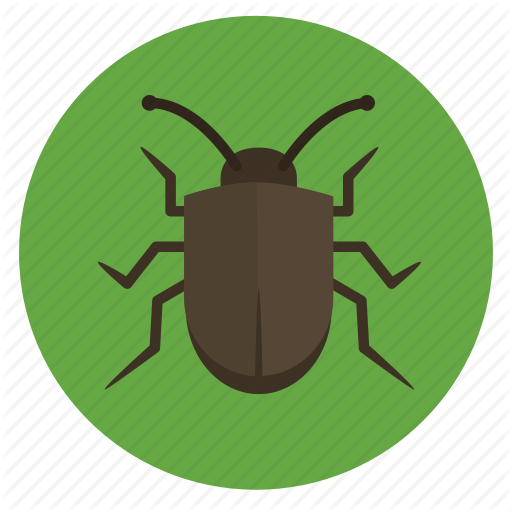
\includegraphics[width=\paperwidth]{sambug}}
	\end{center}
	
	%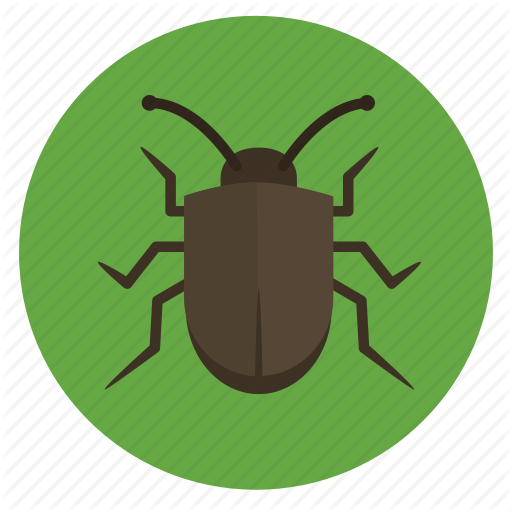
\includegraphics[width=\paperwidth]{sambug}
	
    \vspace*{2cm}
      \Huge \textbf {SAMBUG}\\
      
    \vspace*{-0.5cm}
	  \huge \textbf {User Manual}\\
	  \hfill\\
	\vspace*{-0.5cm}  
      
\includegraphics[scale=0.2]{logo}\hfill
	
\includegraphics[scale=0.2]{sambug_logo}
         
    \vskip2cm
          
    \large \textbf{\monthyeardate\today}
  
    \vfill
\begin{tabular}{lr}
        	Abrie van Aardt&13178840\\
		Werner Mostert&13019695\\
		Kale-ab Tessera&13048423\\
		Keagan Thompson&13023782\\
		Michelle Swanepoel&13066294\\
	\end{tabular}
\end{titlepage}
	
	

\tableofcontents

\pagebreak

\section{System Overview}
\subsection{Introduction}
SAMBUG is a system that will ease the process of stinkbug pest scouting on a farm. Features of the system include stinkbug classification and recognition, data storage, reporting on various scouting trips and more.
\subsection{Utilisation}
Farmers can use the system in two ways, namely an Android application and a browser interface.\\\\
The way in which the system will help farmers will be listed below:
	\begin{itemize}
		\item Farmers can easily use the Android application to classify stink bugs (during a scouting trip). Classification can be done using two methods, manual classification and automatic classification:
		\begin{itemize}
			\item \textbf{Manual Classification:} This method allows the user to take a photo of a single bug and compare it with various other photos taken from a pre-selected gallery of photos. The user will select the photo that most resembles the bug that he/she wants to classify.
			\item \textbf{Automatic Classification:} This method also allows the user to take a photo of the specific bug, and thereafter the application will do the classification by using an artificially intelligent system. 
		\end{itemize}
		\item While scouting and classifying bugs, the application makes it easy to enter additional data, such as the number of that specific bug that was found, in which block of the farm it was, etc.
		\item After doing a scout trip, a summary will be shown, summarising the number and types of bugs found during that trip. Using this summary, farmers can decide with more confidence if spraying pesticide is necessary or not.
		\item When taking a photo during classification, the geolocation will be taken as well. With this feature, farmers will find it easier to make sure that scouts actually go out to random locations.
		\item After capturing the data for a scout trip, this data will be stored in a database such as to later look back at the data.
		\item The browser interface will offer various services, of which the most important is reporting services based on previous scouting trips.
		\item Administrators at Subtrop will be able to view data from different farms to also help them reach conclusions.
		\item On the browser interface it will be possible to enter data concerning pesticide spraying. This will also be stored in the database and may later be used to view data.
	\end{itemize}
	
\subsection{Intended Audience}
The intended audience of this systems is farmers specifically dealing with stink bugs as pests on their farms. Any farmer who seeks assistance with regards to bug classification, data management and scout trip management will find the system useful. The system will specifically assist farmers who do scouting of pests to reach certain conclusions, such as whether to spray pesticide or not, where and when pests are more, etc.

\subsection{Users}
The system has in mind three different users which will be described bellow:
	\begin{itemize}
		\item \textbf{Staff of Subtrop} These users will have access to all data from all the farms using the system. This means that when they log on in the browser interface they will be able to generate reports based on collective data from all farms.
		\item \textbf{Farmers} Farmers will use the browser interface, but may also use the Android application. Farmers will only be able to generate reports based on data from their own farm, thus other farms' data will not be visible. 
		\item \textbf{Scouts} Scouts will mainly use the Android Application to enter data and do classifications while in the field. The Android application is developed to keep in mind different language preferences, thus minimum usage of actual words and more symbols to carry over a message.
	\end{itemize}



\section{System Configuration}
Before we go into any further detail, it is important to ensure that you are fully equipped with the necessary prerequisites to enjoy the SAMBUG system. This section outlines everything you need to get started.
\subsection{Setup Overview}
SAMBUG is intended to be an integrated solution. The Android application and Website are complementary. Figure \ref{fig:layout} depicts the common high-level configuration of the system. Please note that Figure \ref{fig:Web} may be interchanged with any Web-enabled device.
	\begin{figure}[h]
		\begin{subfigure}{0.3\textwidth}
			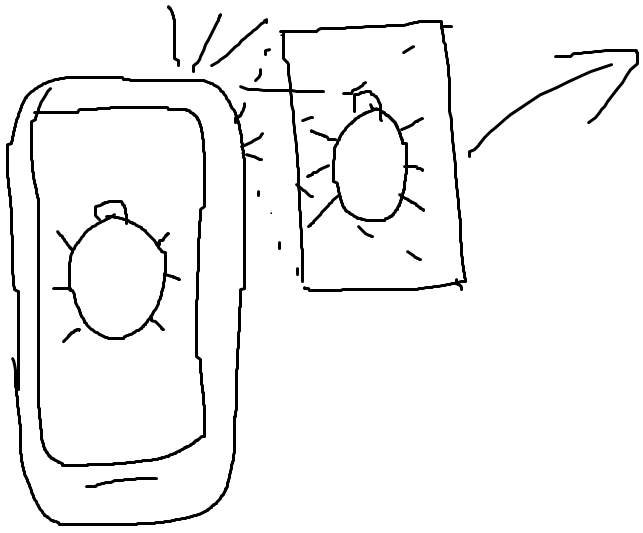
\includegraphics[width=0.9\linewidth]{Fig1a}
		\caption{Data Capture}		
		\label{fig:dataCapt}	
		\end{subfigure}
		\begin{subfigure}{0.3\textwidth}
			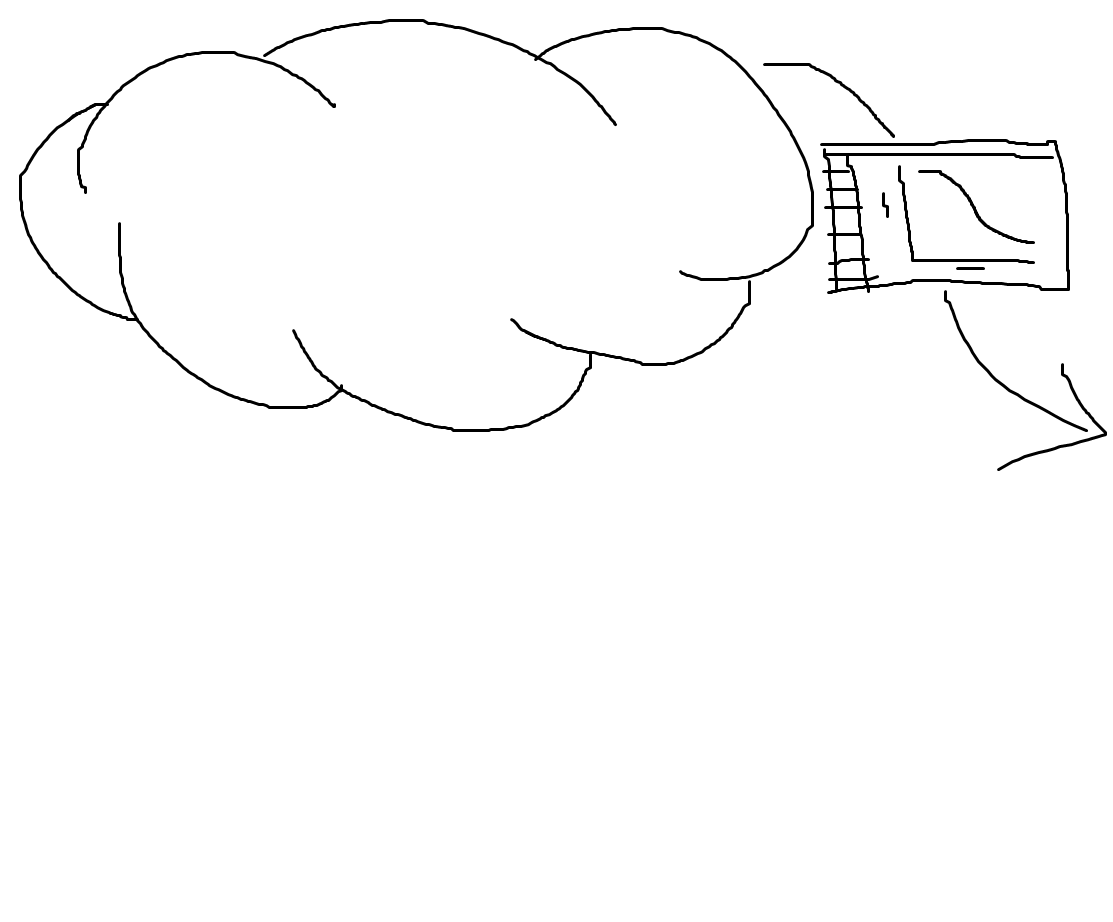
\includegraphics[width=0.9\linewidth]{Fig1b}
		\caption{History \& Analysis}		
		\label{fig:Engine}	
		\end{subfigure}
		\begin{subfigure}{0.3\textwidth}
			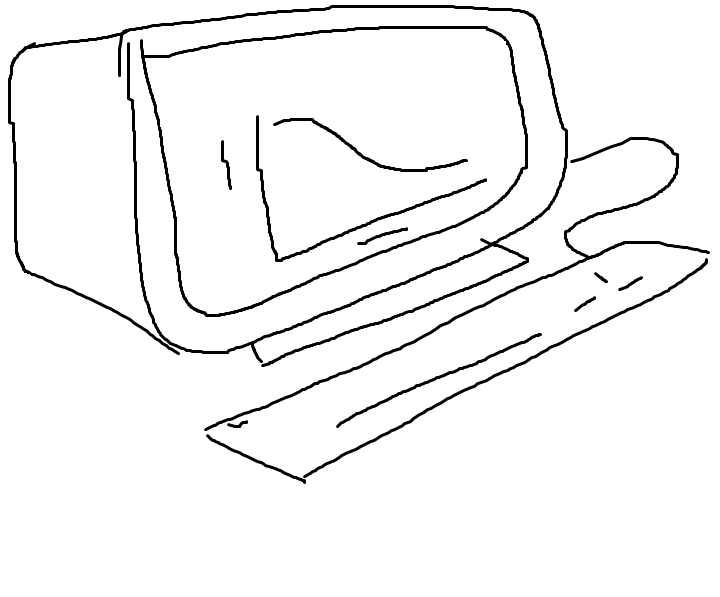
\includegraphics[width=0.9\linewidth]{Fig1c}
		\caption{Farm Management \& Consolidation}	
		\label{fig:Web}		
		\end{subfigure}
	\caption{Illustration of SAMBUG's Configuration}
	\label{fig:layout}
	\end{figure}

\subsection{Hardware \& Software Requirements}
The design of the system as indicated above lends itself to a number of required devices and services, including:
	\begin{itemize}
		\item An Android Smartphone or Tablet \footnote{You are advised to use a device with a camera that's able to take good quality macro photos in a medium level of light} (Android 4.1 or higher) - This will house the application used during Scouts, your main access point to the system.
		\item A Second Web-enabled device - This is where you will manage your farm and view consolidated information of your scouts. Although you may choose to use the same phone/tablet you use in the field, the Web-based nature of this part of the system will allow you to work on a device with a large display, suitable for office work (e.g. a PC).
		\item An Internet Browser - Whatever your choice of device in Figure \ref{fig:Web}, it must have one or more of the latest (As of \monthyeardate\today) popular Internet Browsers installed. You may choose from an extensive list, including, but not limited to:
		\begin{itemize}
			\item Google Chrome
			\item Internet Explorer/Microsoft Edge
			\item Mozilla Firefox
			\item Safari
		\end{itemize}
		\item An Internet Connection - Our application is designed to perform all of its functions even where no mobile/WiFi network reception is available. However, the information you'll be gathering during your scouting trips will have to be uploaded to the server at some point, and for that, you need to be connected to the internet. 		
	\end{itemize}

\section{Installation}
The Android application will be available for download via the Google Play Store. The web application will be permanently available via the internet at \url{http://sambug.azurewebsites.net}.\\

Alternatively, the full source code may be accessed from the public GitHub repository at \url{https://github.com/WMostert1/Vector-Software-Developers}. In order to build and obtain the source code, some technical knowledge is required. To download the source code directly, navigate to the previously mentioned GitHub URL and click on [Download ZIP].

	\begin{center}
		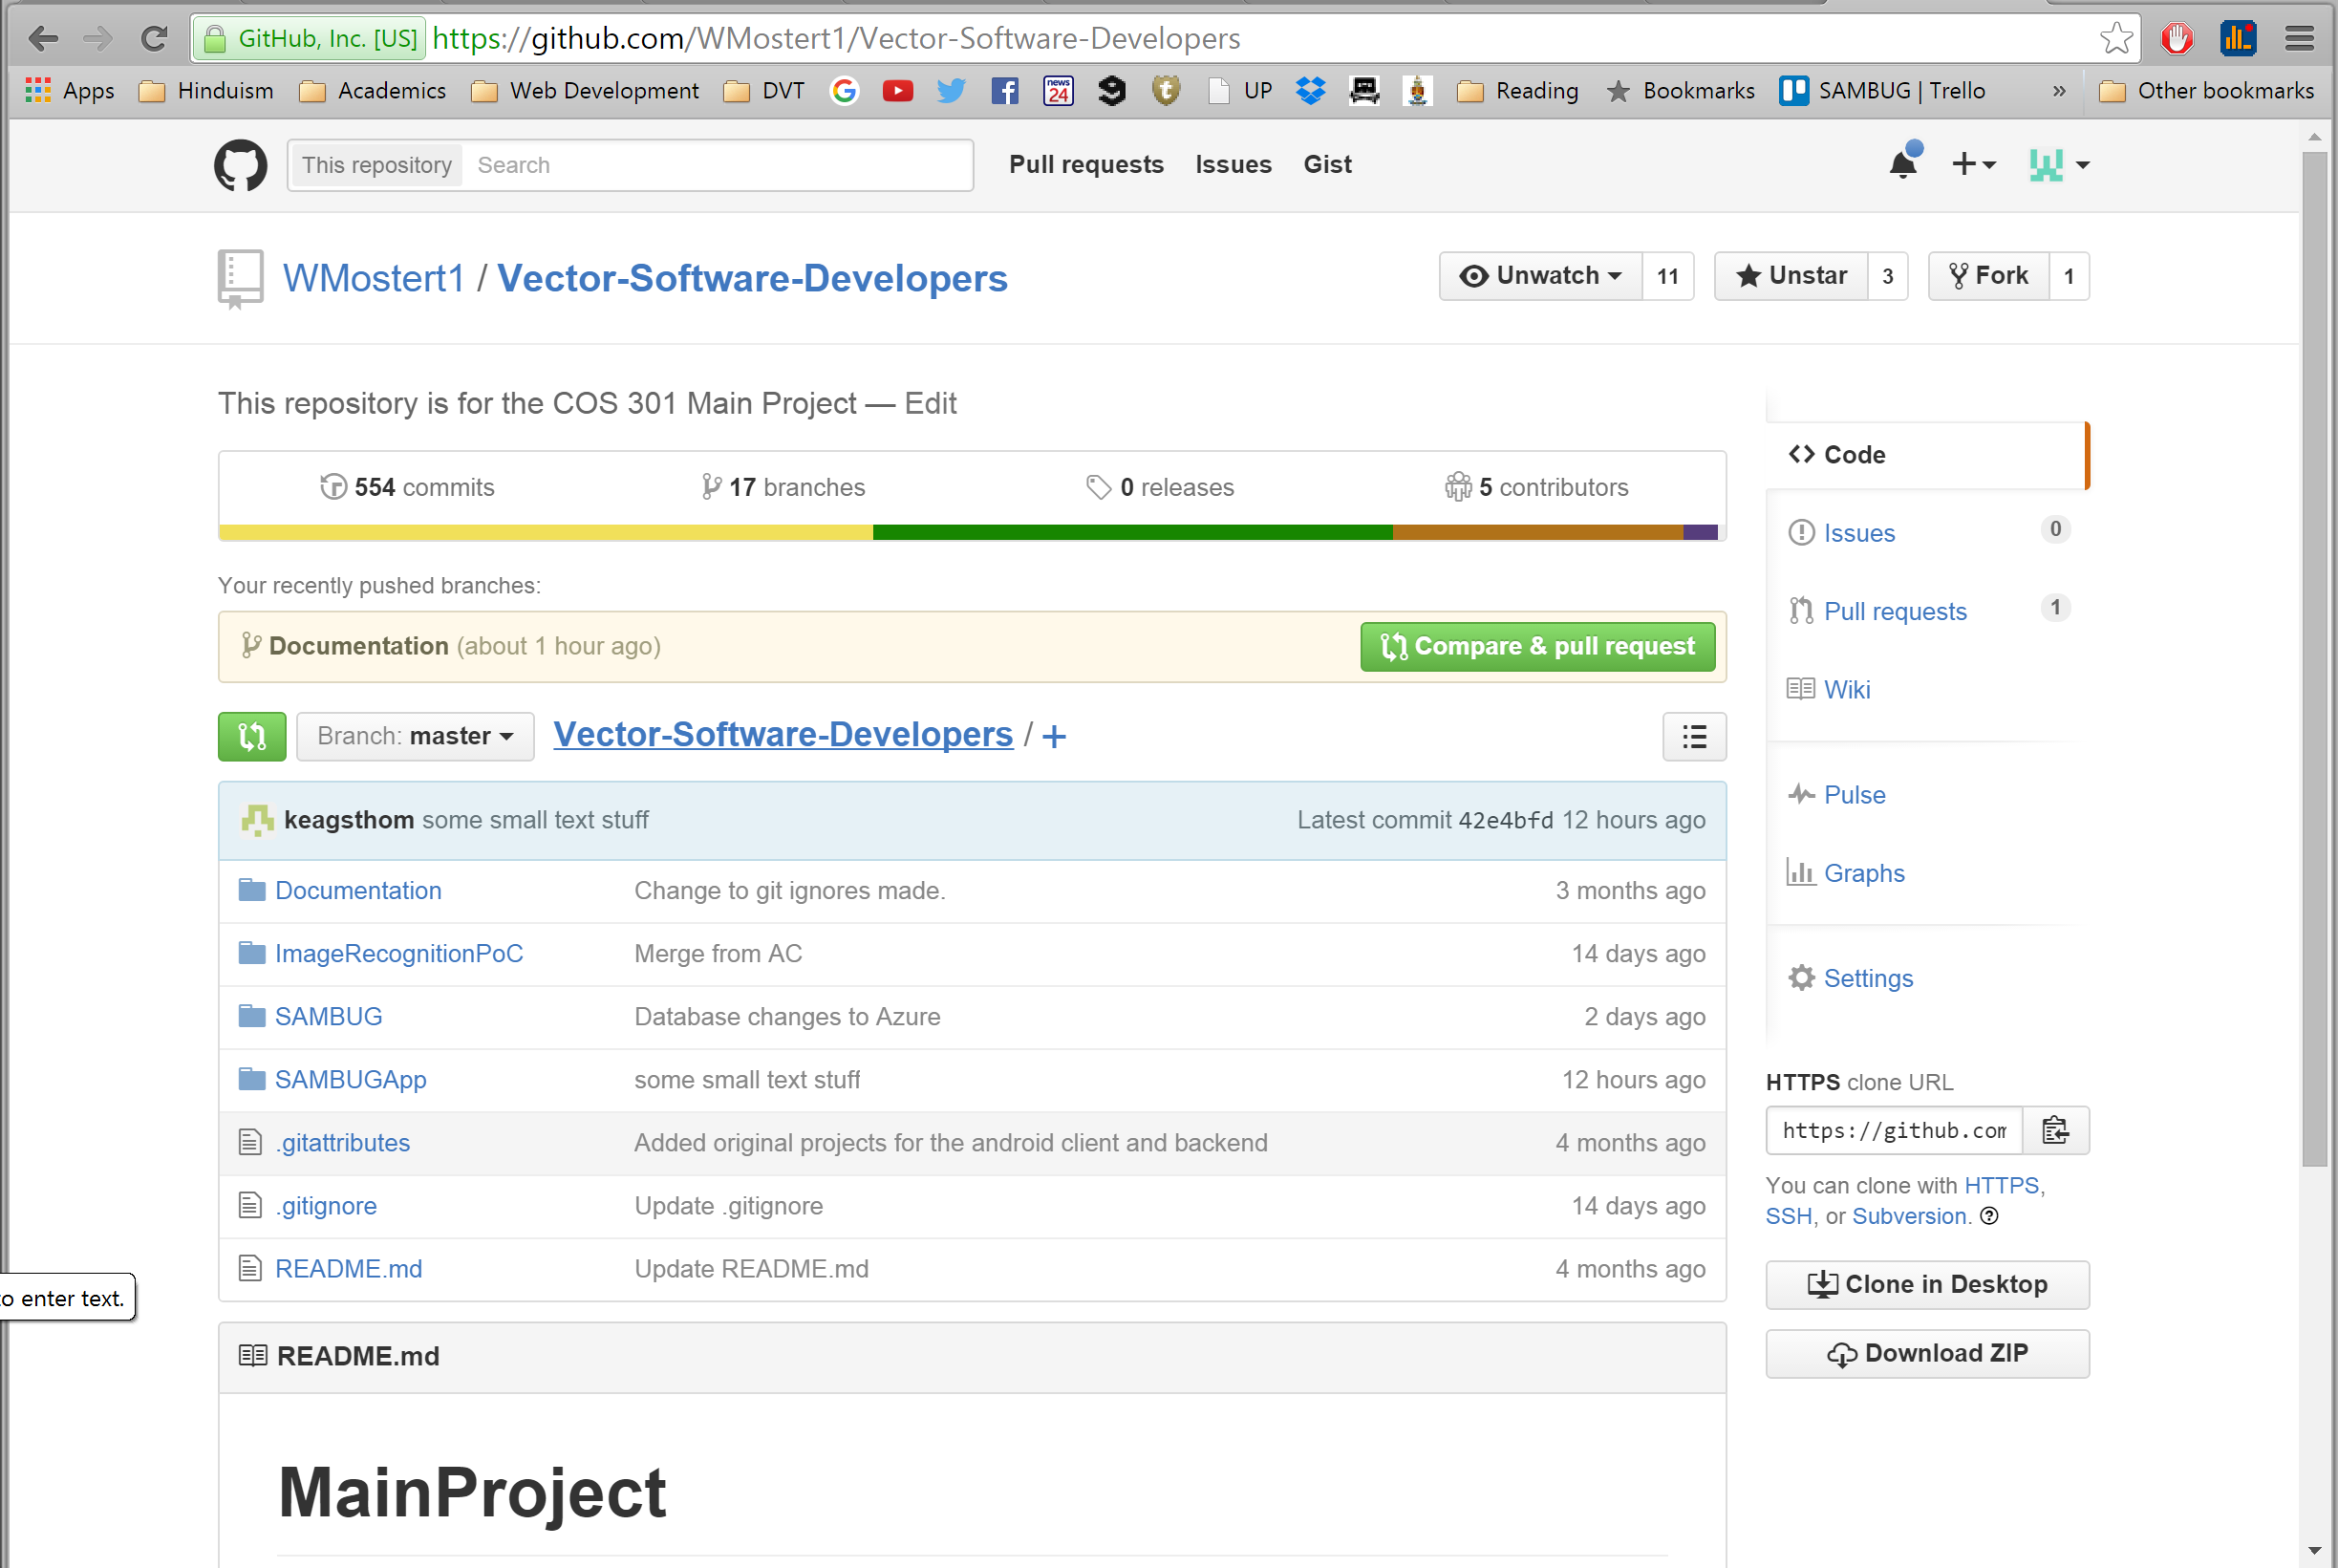
\includegraphics[width=\linewidth]{git.png}
	\end{center}

Once the source code has been downloaded successfully, there are two different projects within the folder. SAMBUG is the web-backend. To open and run the project, install/open Microsoft Visual Studio 2013 and open the .sln file located within the SAMBUG folder.\\
In order to run the Android Application, open the SAMBUGApp project using Android Studio 1.2.\\
In both cases, all dependencies should be automatically installed to your computer via Gradle (for Android Studio) and NuGet (for Visual Studio). 
		
\section{Getting started}
\subsection{Requirements to access the system}
In order for a user to use the system, it is necessary that he/she registers as a user first. This can only be done on the web page. Only an email address and password will be asked for at registration. A user can only become a privileged user if another privileged user authorises him/her. Farmers and scouts will use the same account, and thus the same credentials to use the system.\\
After registration the user can log in on the Android Application as well as the web page. A user logged in to the Android application will stay logged in if he/she does not explicitly log out. The details used to log in are only the email (as a username) and password.

\subsection{System Overview}

\textbf{\textit{Please see Using the System section for detailed system flow and usage.}}\\

The general flow of the system:
	\begin{center}
		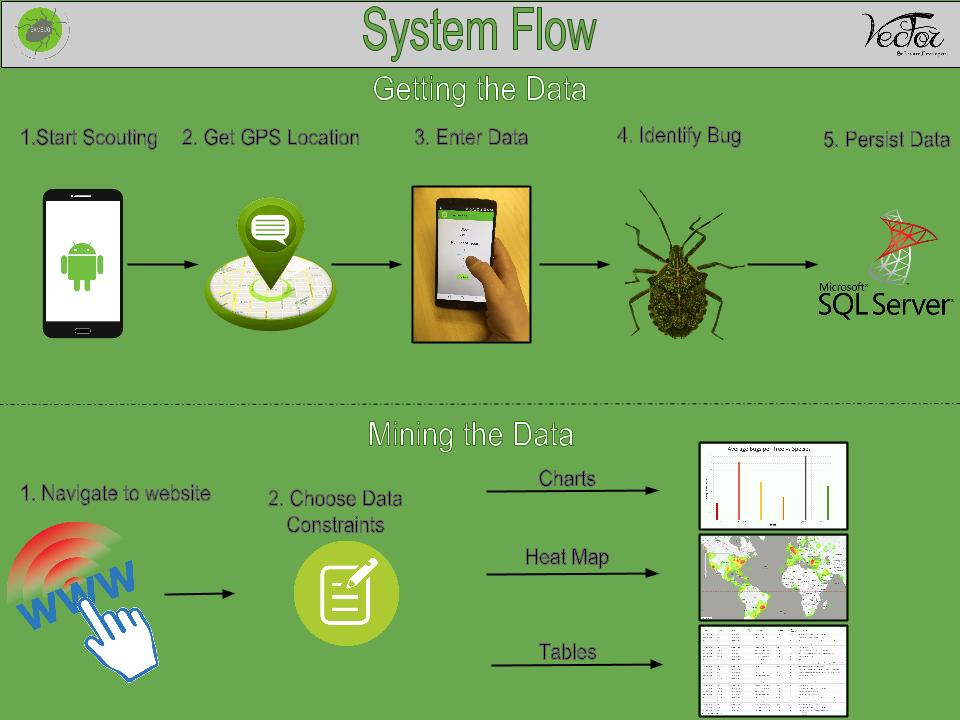
\includegraphics[width=\linewidth]{SystemFlow.jpg}
	\end{center}

If the user is a subtrop staff member, the mobile application will not be used, only the web interface since administrators will not originate data. Due to this fact, the work flow differs between Growers and Administrators.
\section{Using the System}
\subsection{Web Page}
		 The Web Application's main goal is data mining and various management responsibilities. Complete the following walk-through in order to utilise the system:
	\begin{enumerate}
		\item Navigate to \url{http://sambug.azurewebsites.net}
		\item If you are already registered please login, if not click on "here" to register and refer to Step 4 of this section for farm setup instructions. If you have forgotten your password, click on "here" to recover your account.  %TODO
	\begin{center}
		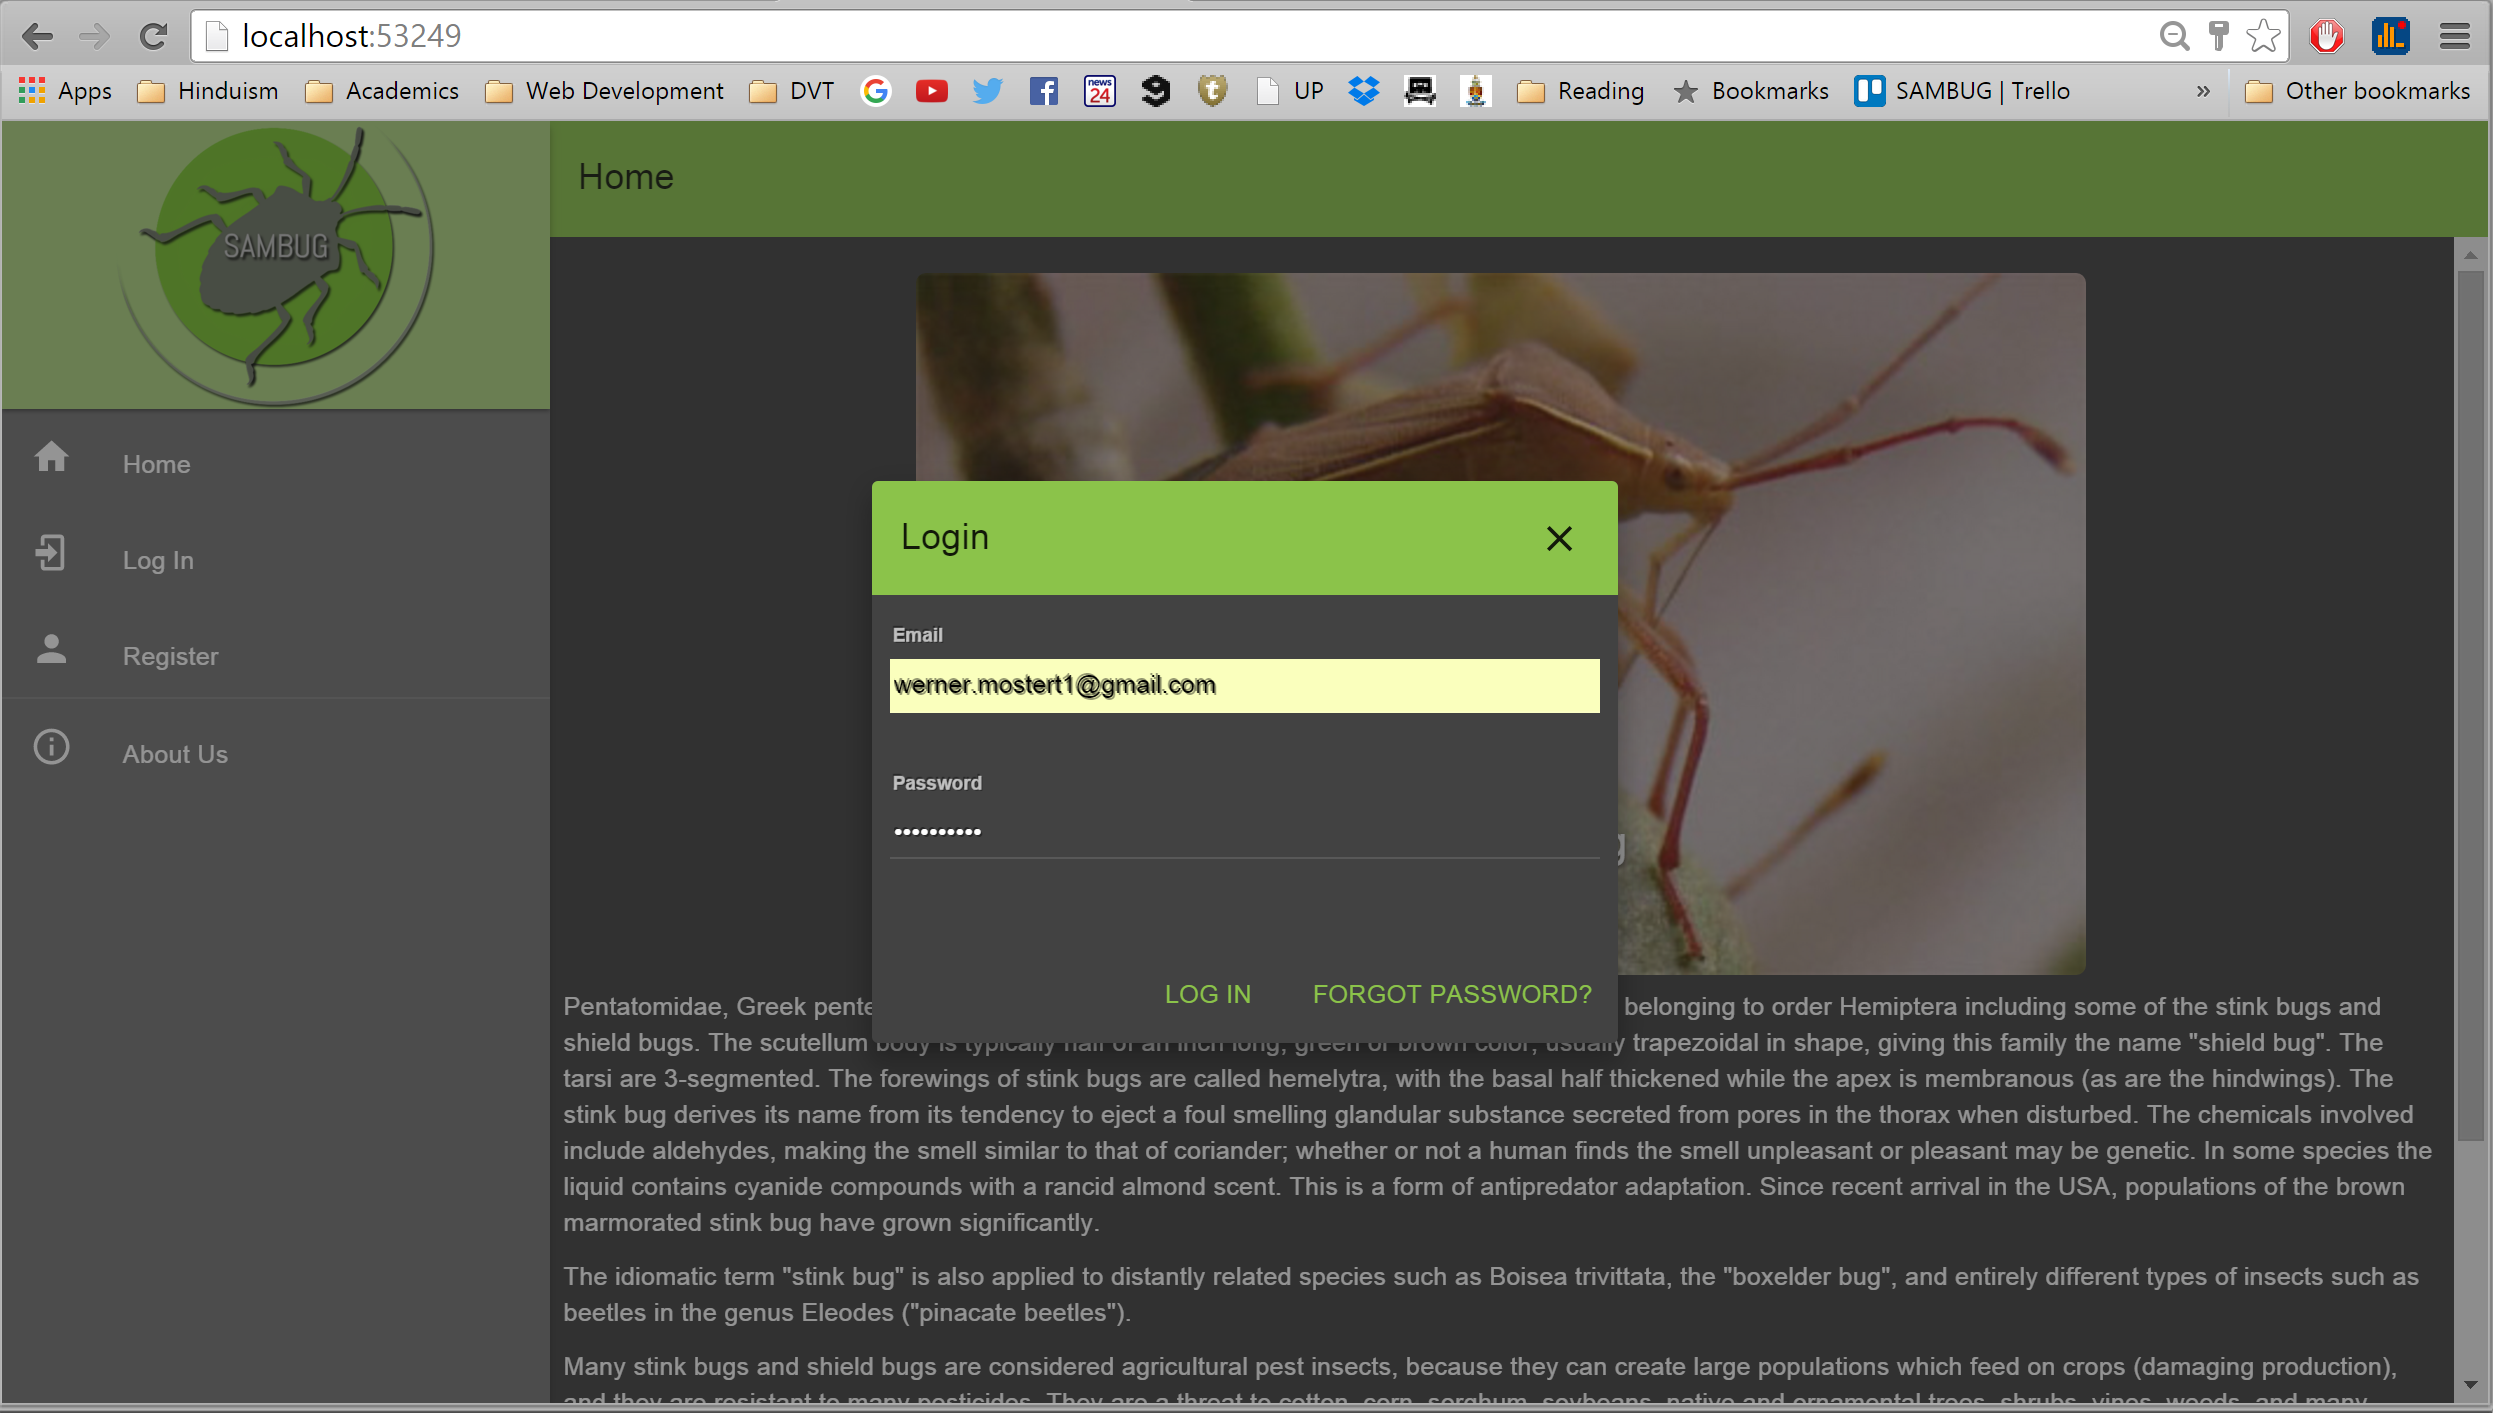
\includegraphics[width=\linewidth]{login_page.png}
	\end{center}
		\begin{enumerate}
			\item If you have logged in continue.
			\item If you need to register, enter the details required on the registration page.
				%\begin{center}
					%\includegraphics{registration_page.png}
				%\end{center}
			\item If you need to recover your account, please enter your email address and click on the link provided in order to reset your password.
		\end{enumerate}
\item Once successfully logged in, you should be able to view your farm's historical data by clicking on either "Charts", "Tables", or "Maps". Use the filters for the individual representation to change and scale the mined data as per preference. By using these filters various representations may be obtained. To access filters click the three dotted button on the top right of the screen.
		\begin{enumerate}
			\item The map as shown below:
			\begin{center}
				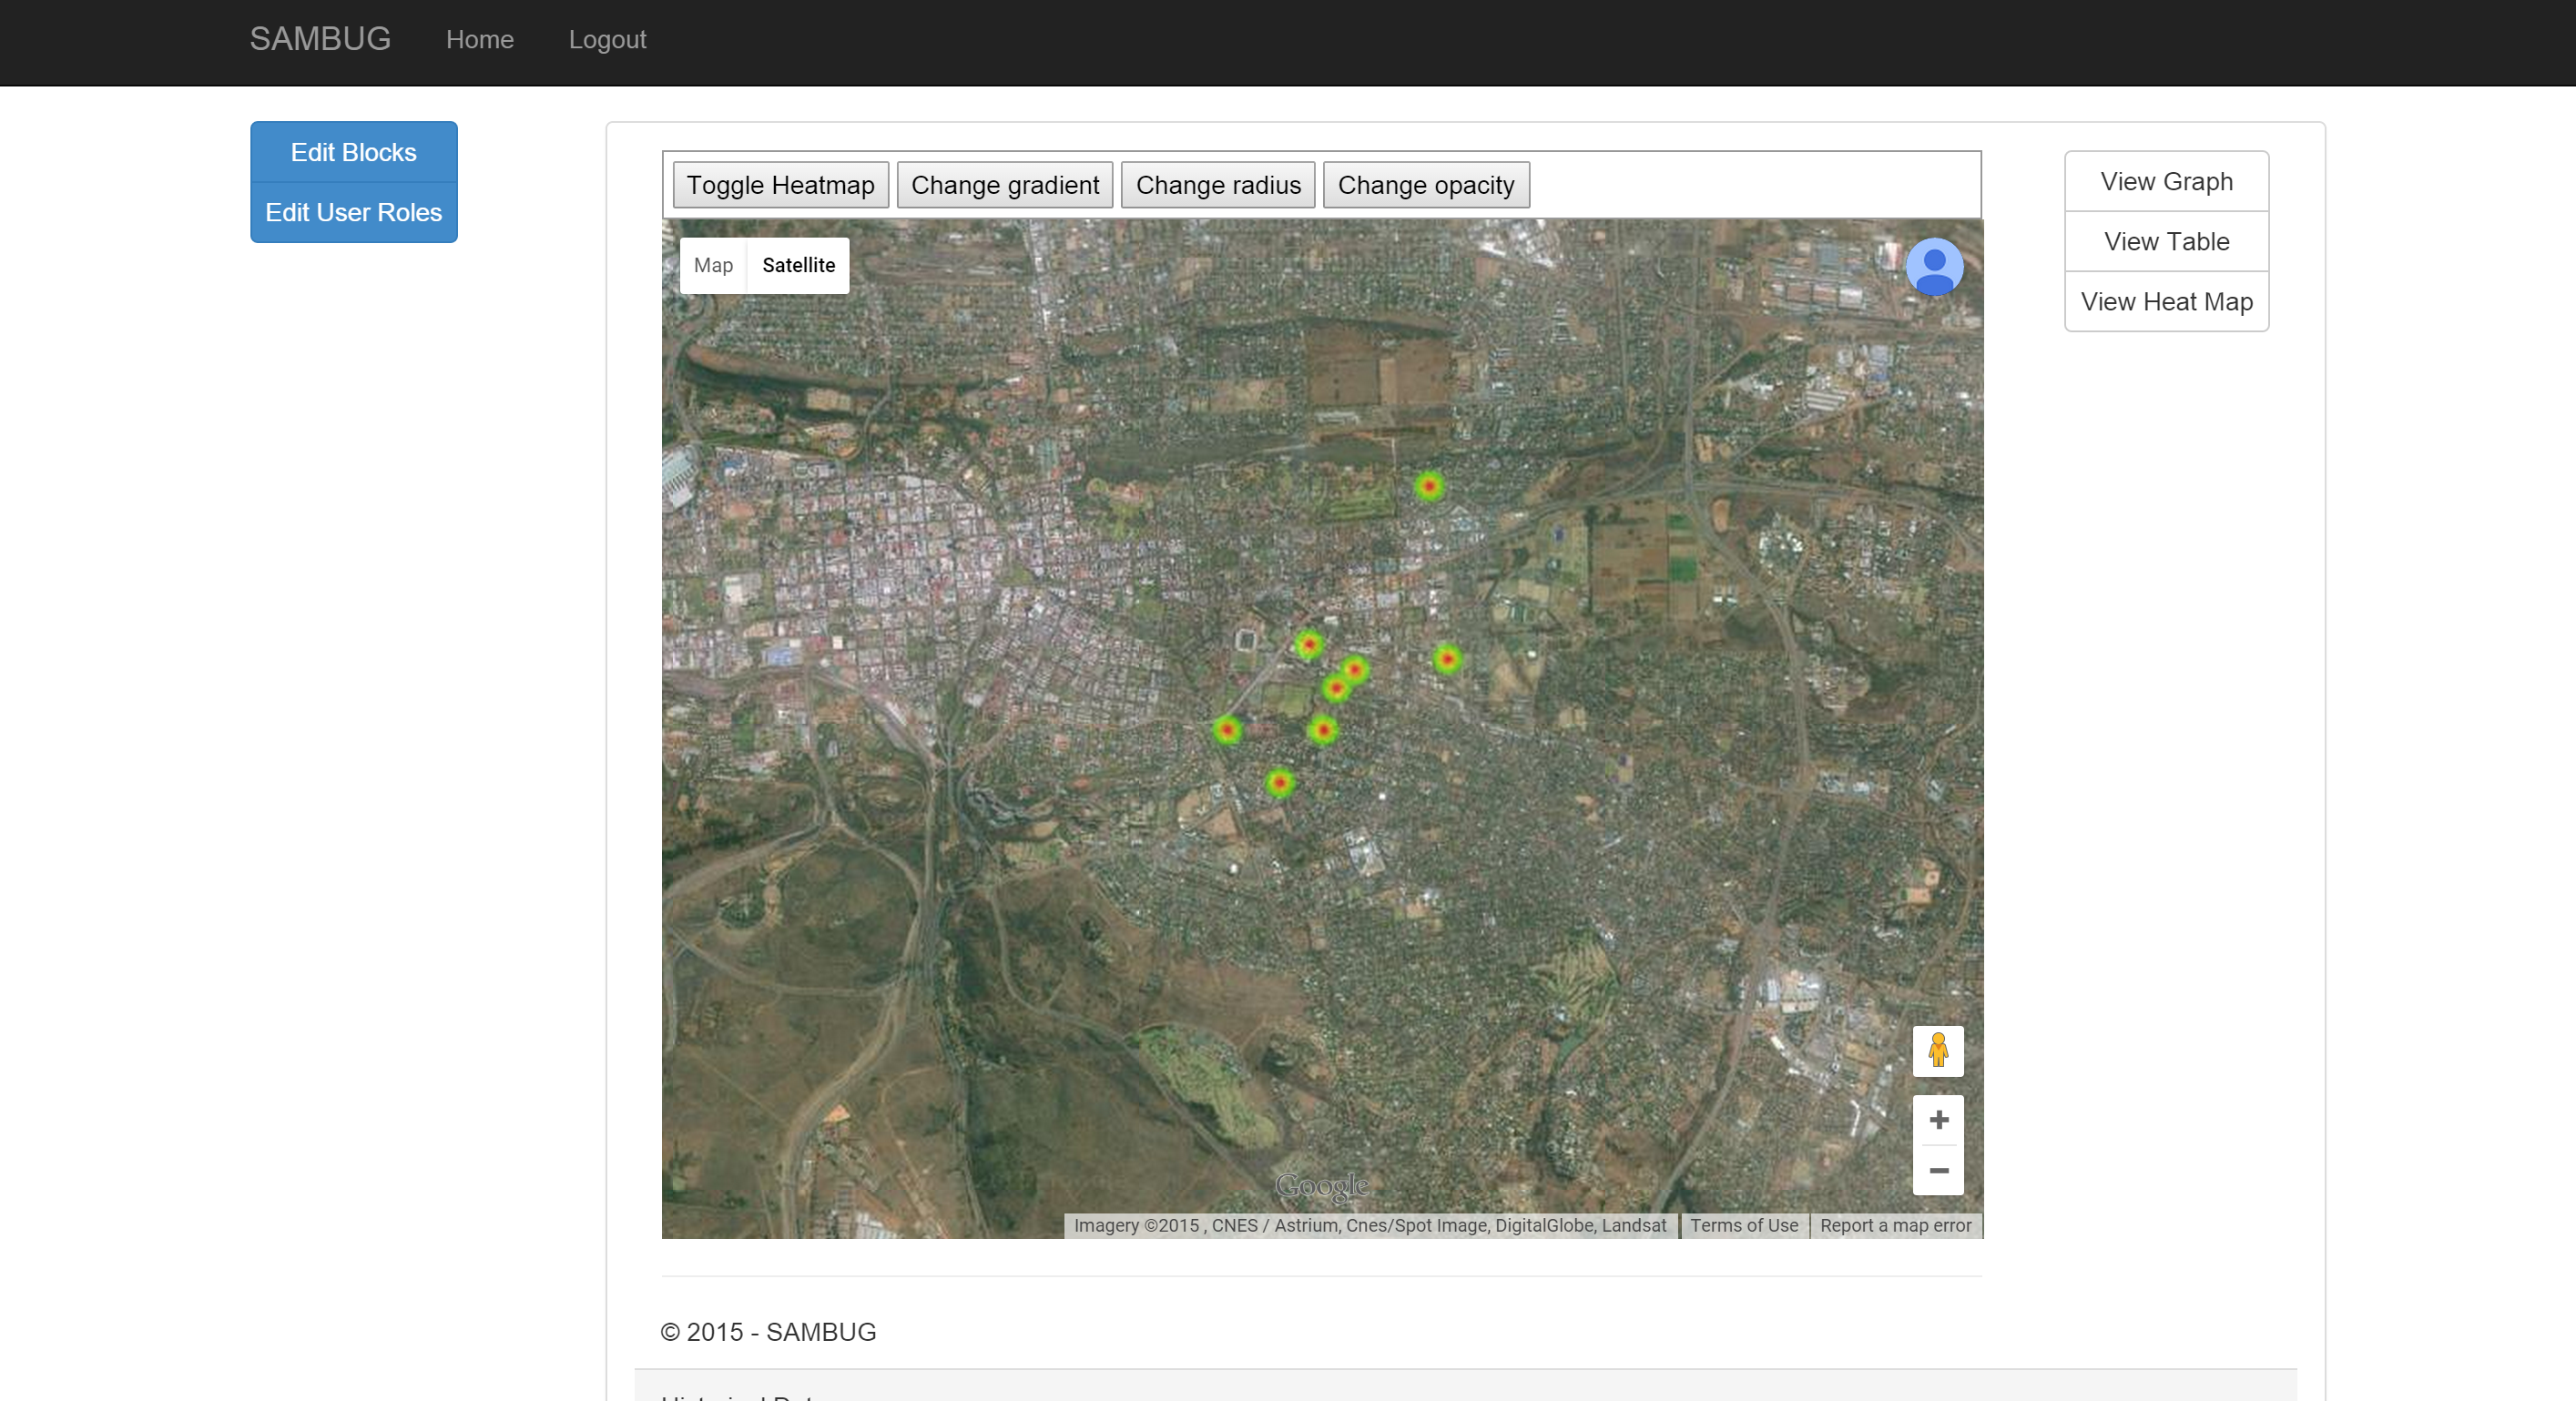
\includegraphics[width=\linewidth]{map.png}
			\end{center}
\item The graph as shown below:
			\begin{center}
				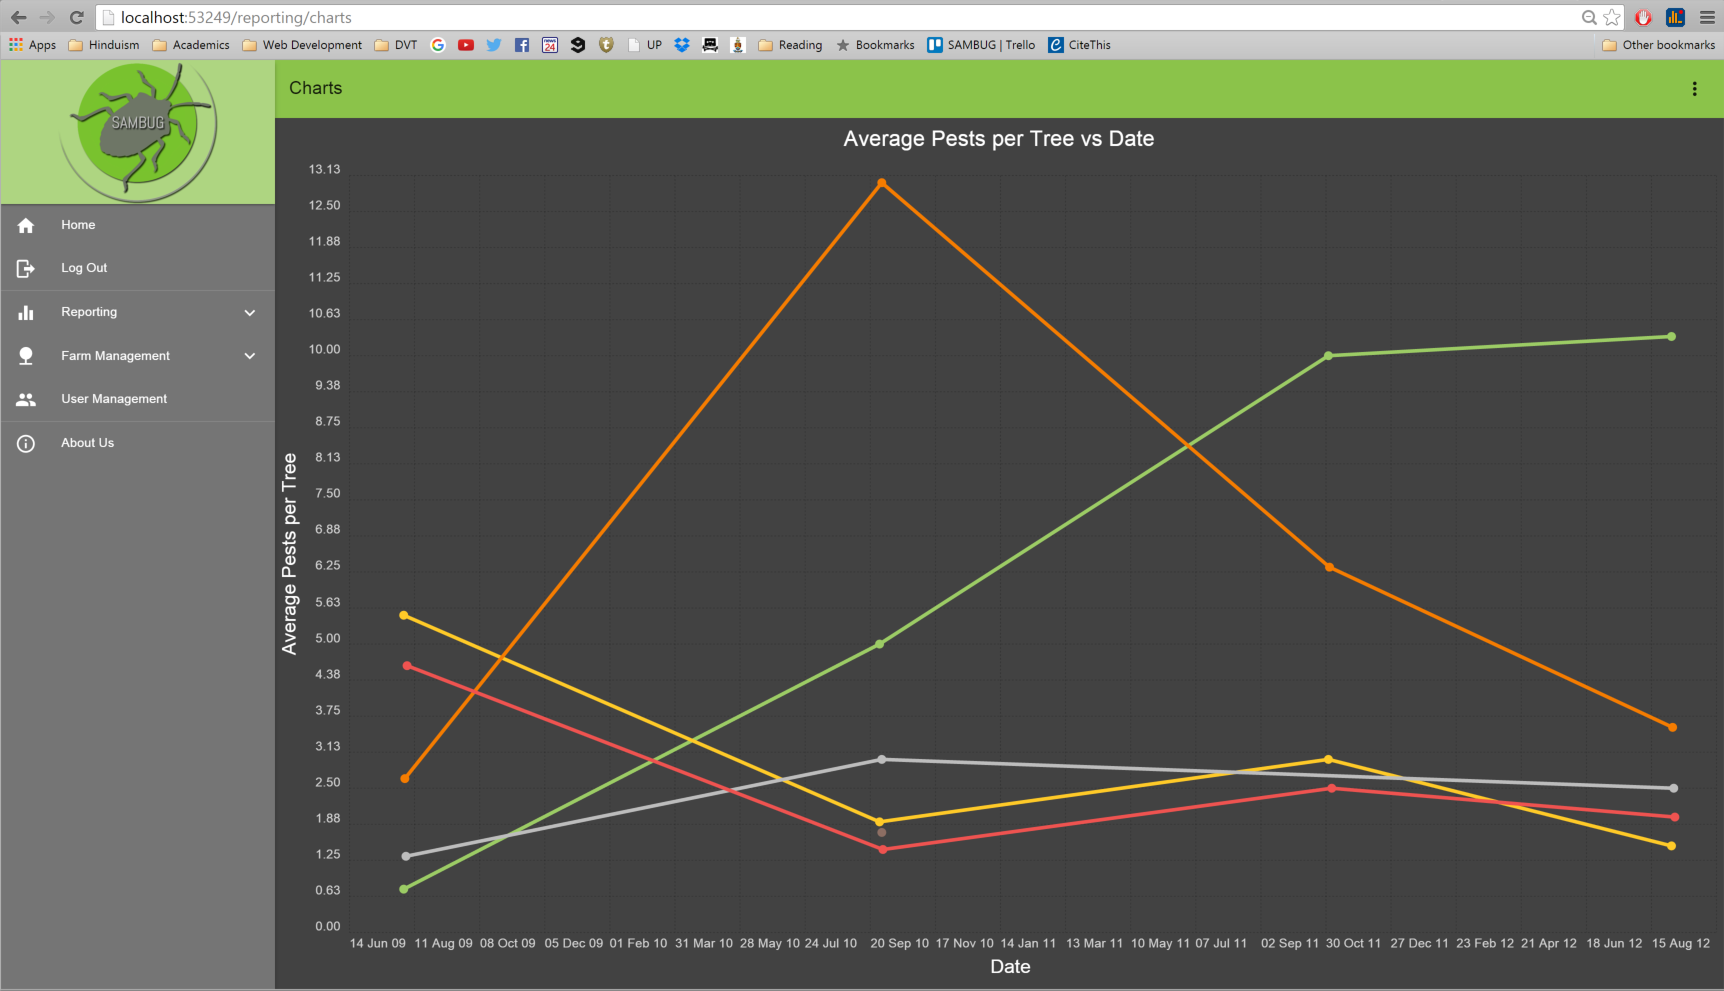
\includegraphics[width=\linewidth]{graph.png}
			\end{center}
\item The table as shown below:
			\begin{center}
				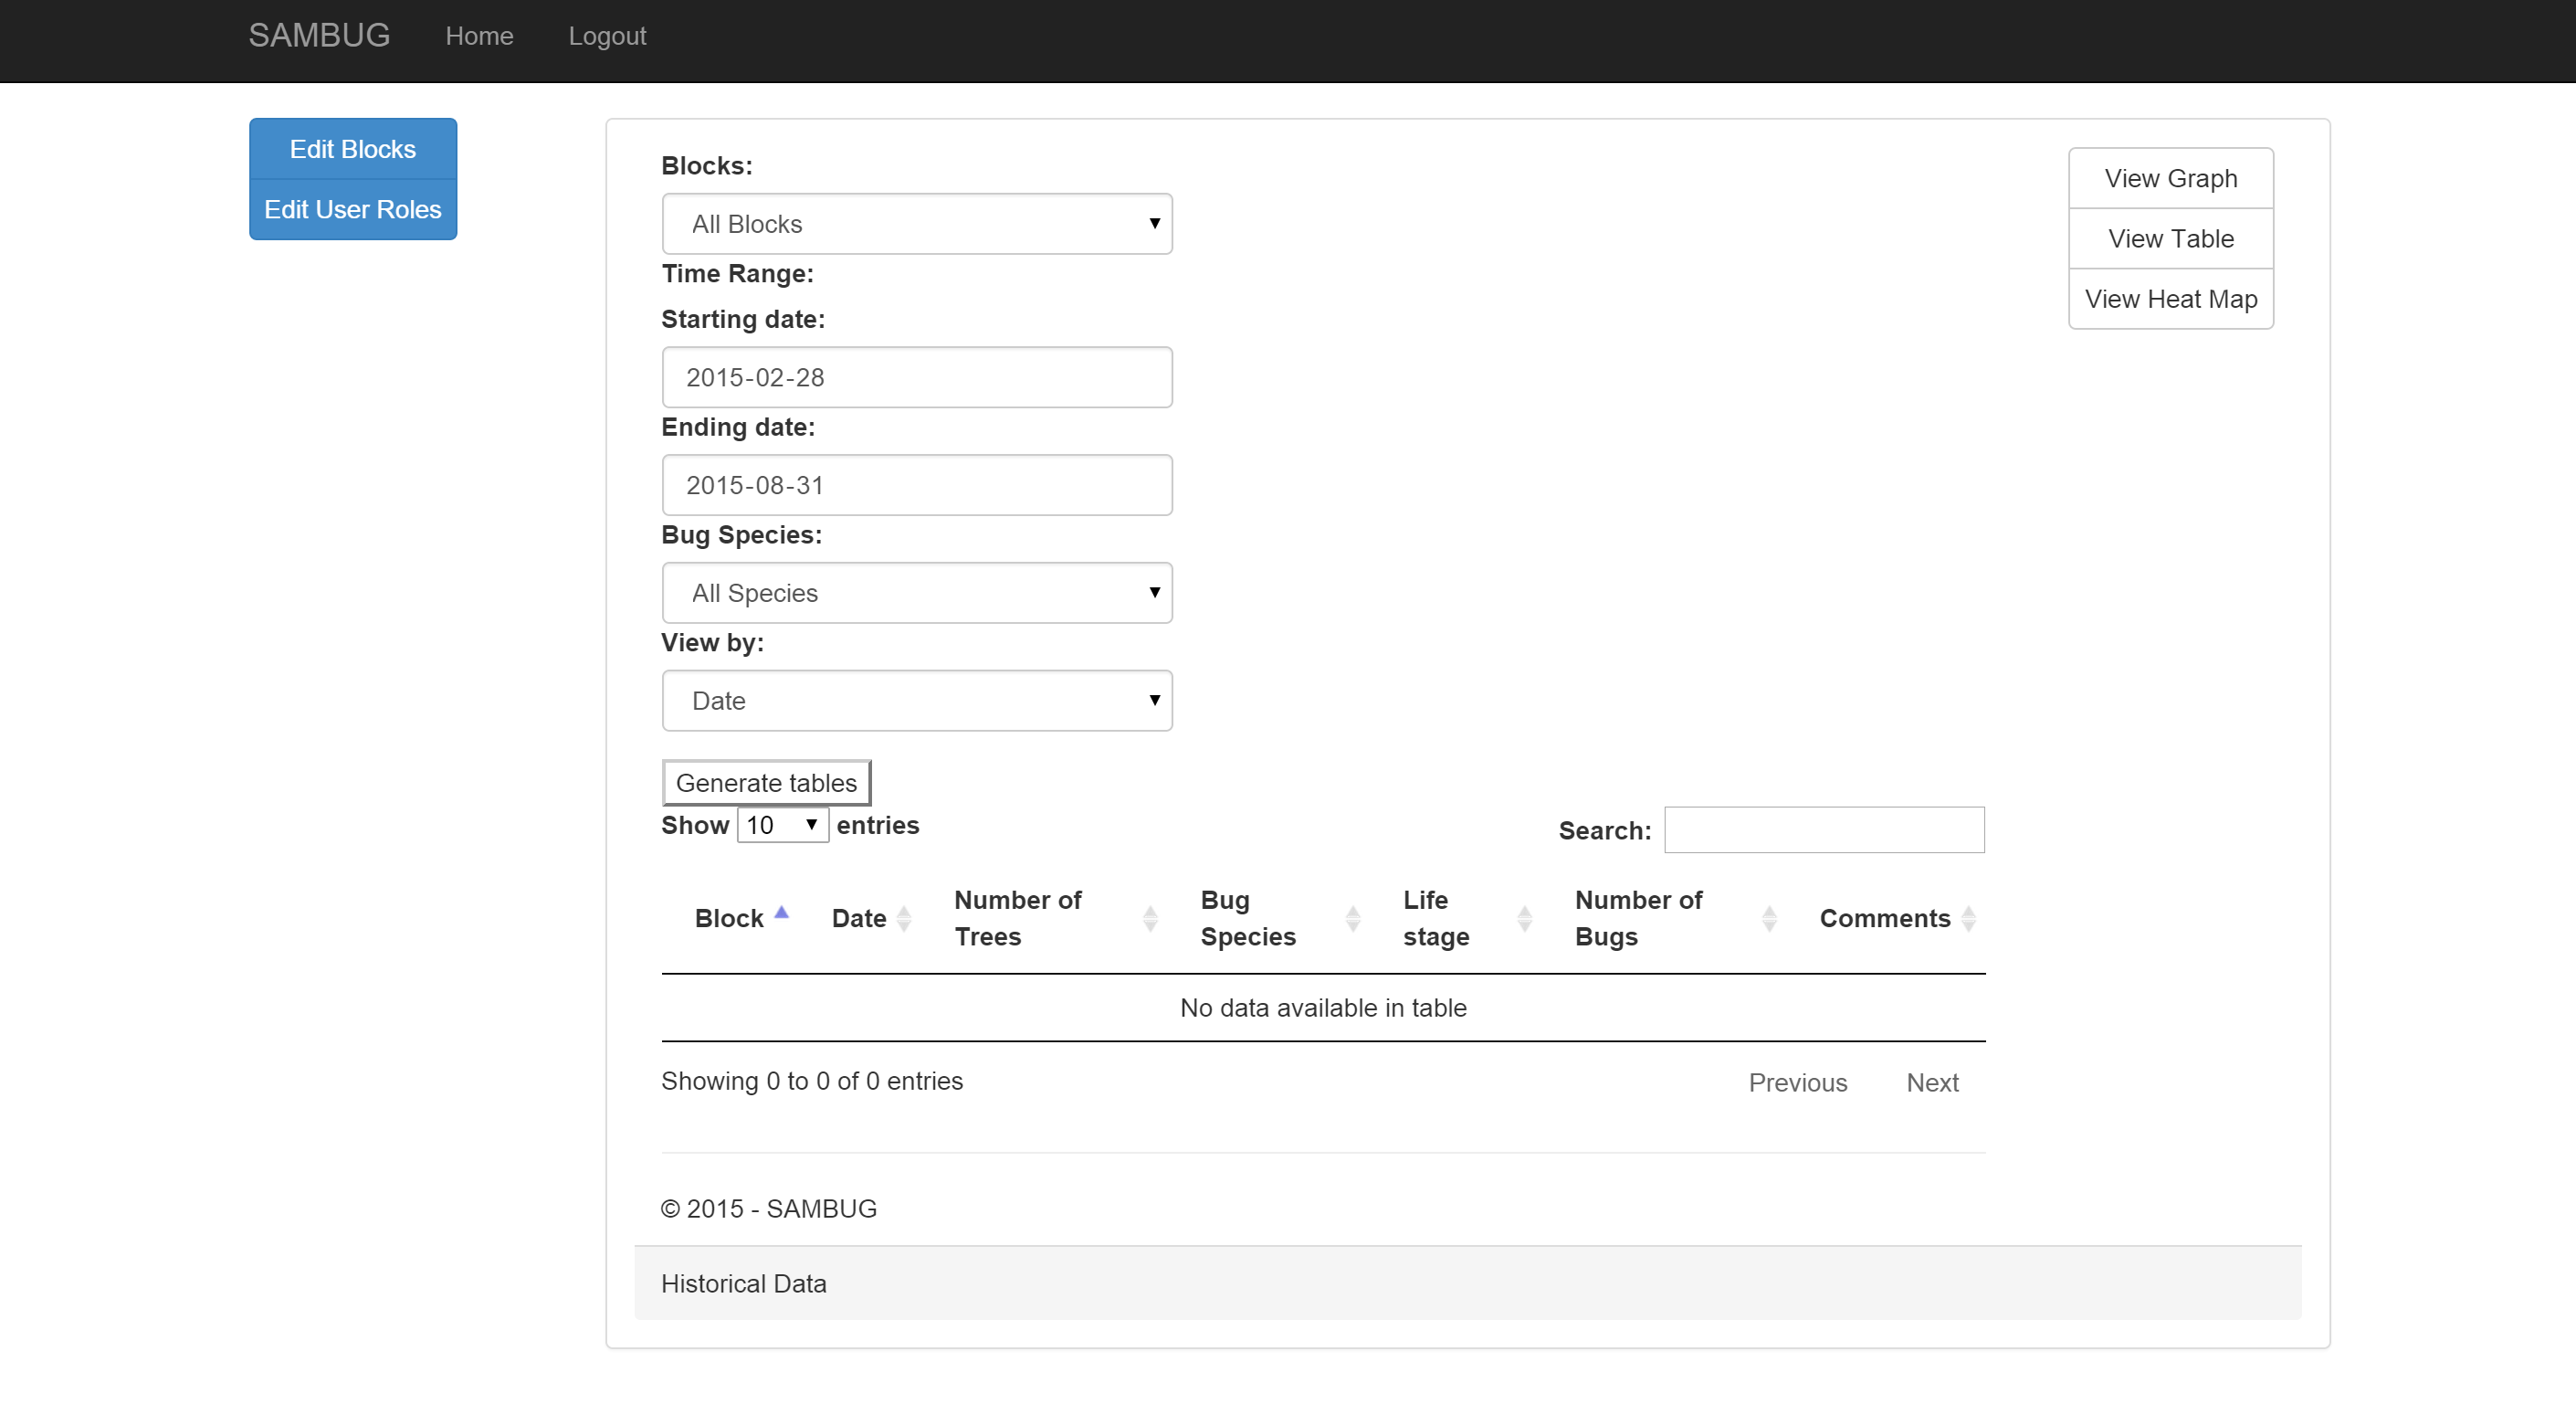
\includegraphics[width=\linewidth]{table.png}
			\end{center}
		\end{enumerate}
\item Once successfully registered, the Grower will need to enter the block structure that he wishes to organise his farm data into using the following page: 
	\begin{center}
		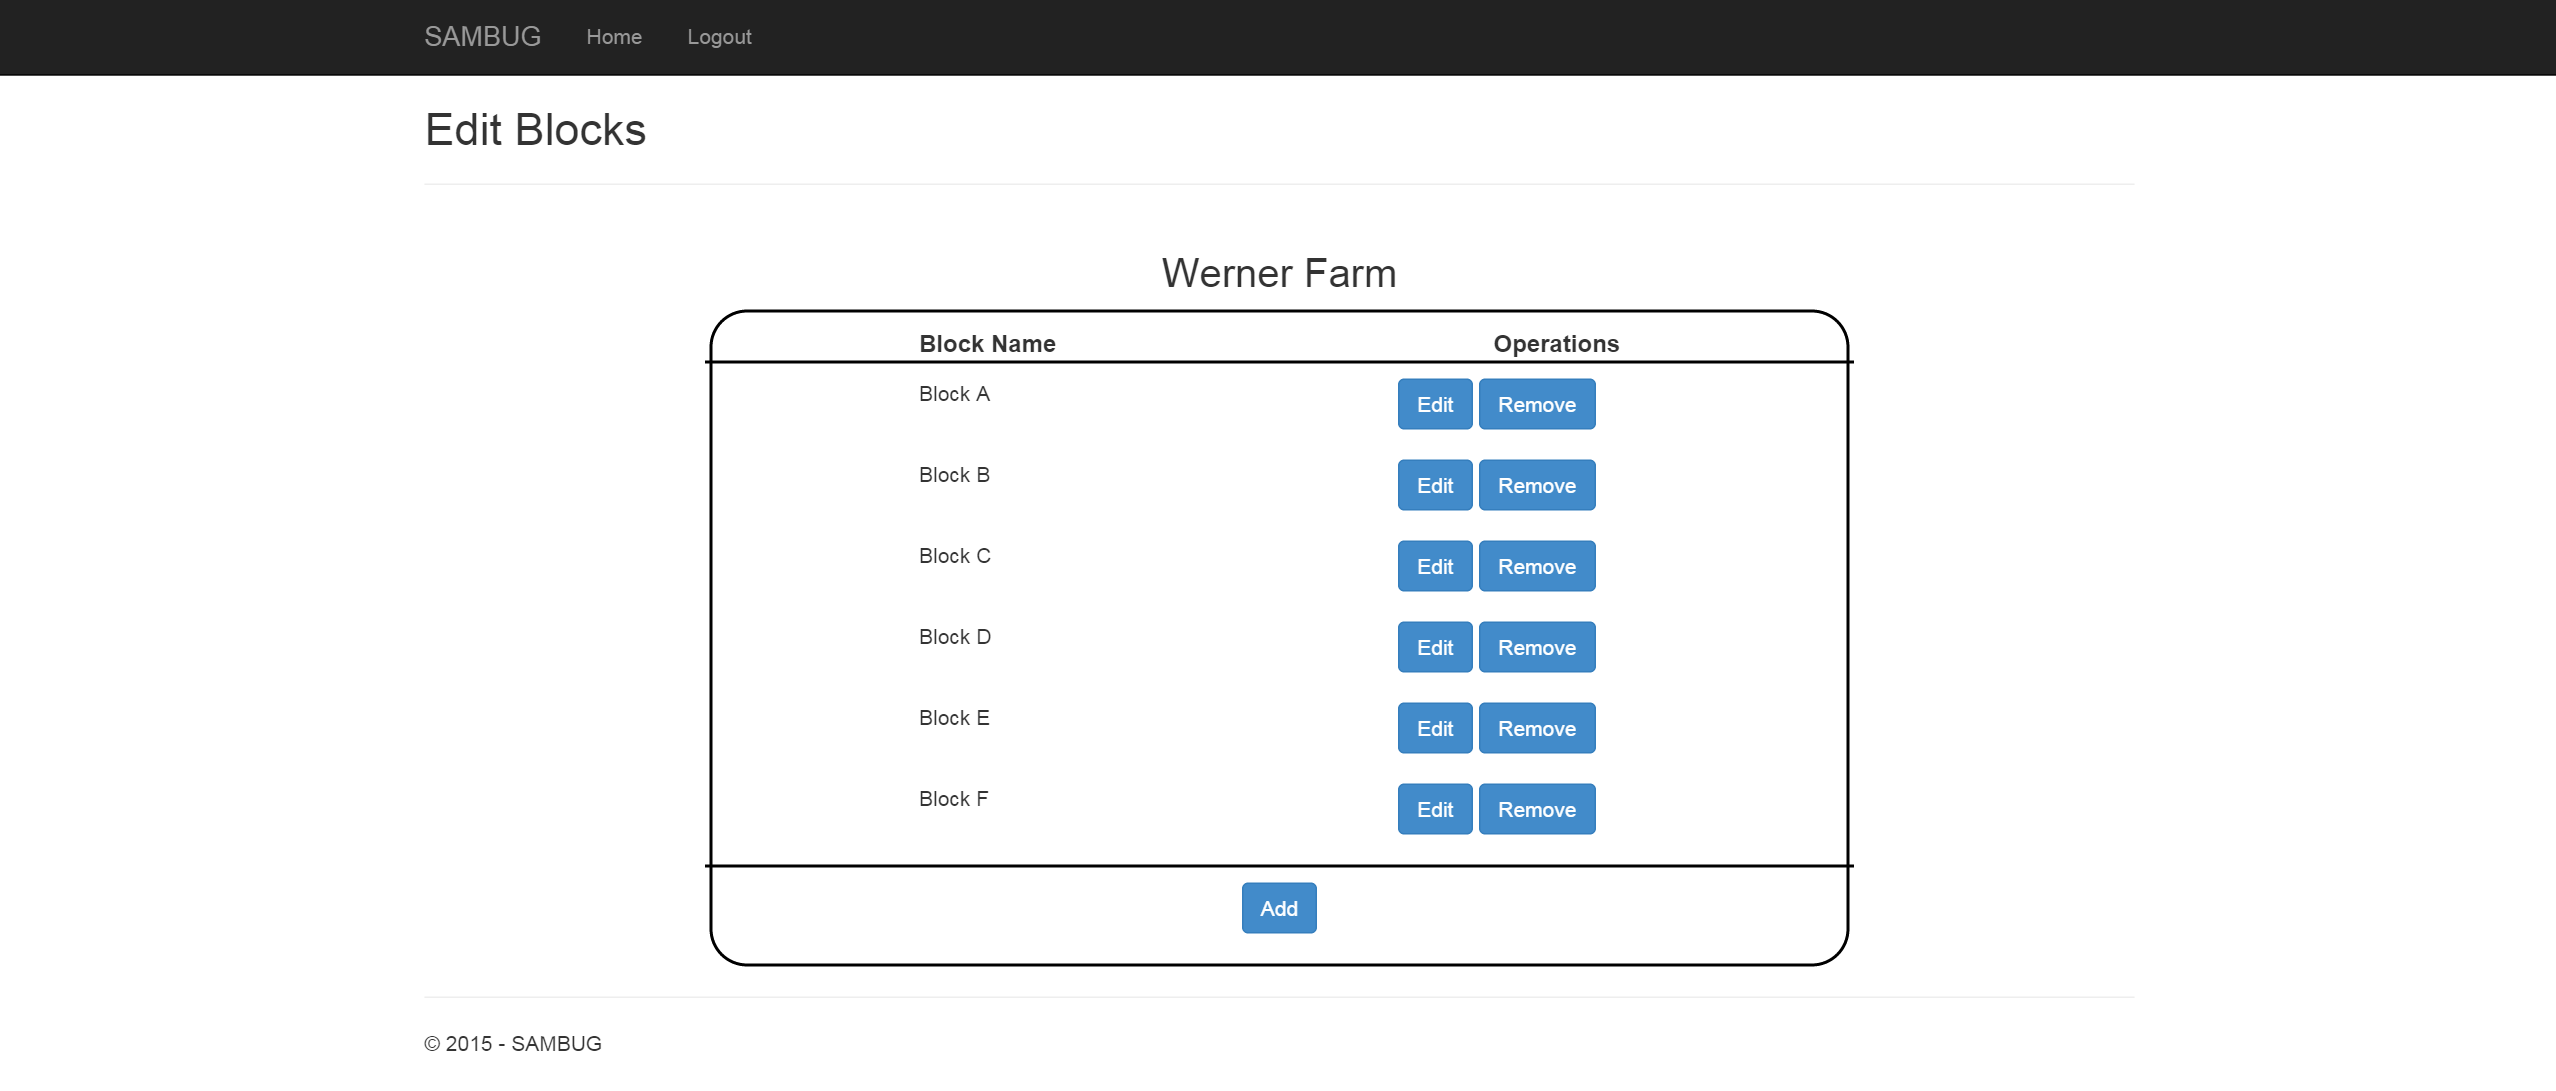
\includegraphics[width=\linewidth]{manageblocks.png}
	\end{center}
	On this page, the Grower has 3 possible options to edit his/her blocks - Add (lower gray plus), Remove (trash can) or Edit (pencil). By clicking appropriate buttons, modal windows will appear for the user to complete each action. Lastly, one may add a new farm to your account by clicking the large green plus.
	
\item Should the logged in user happen to be an Admin, he/she will have access to the Edit User Roles function. By clicking on the appropriate link, the following page will appear: 
	\begin{center}
		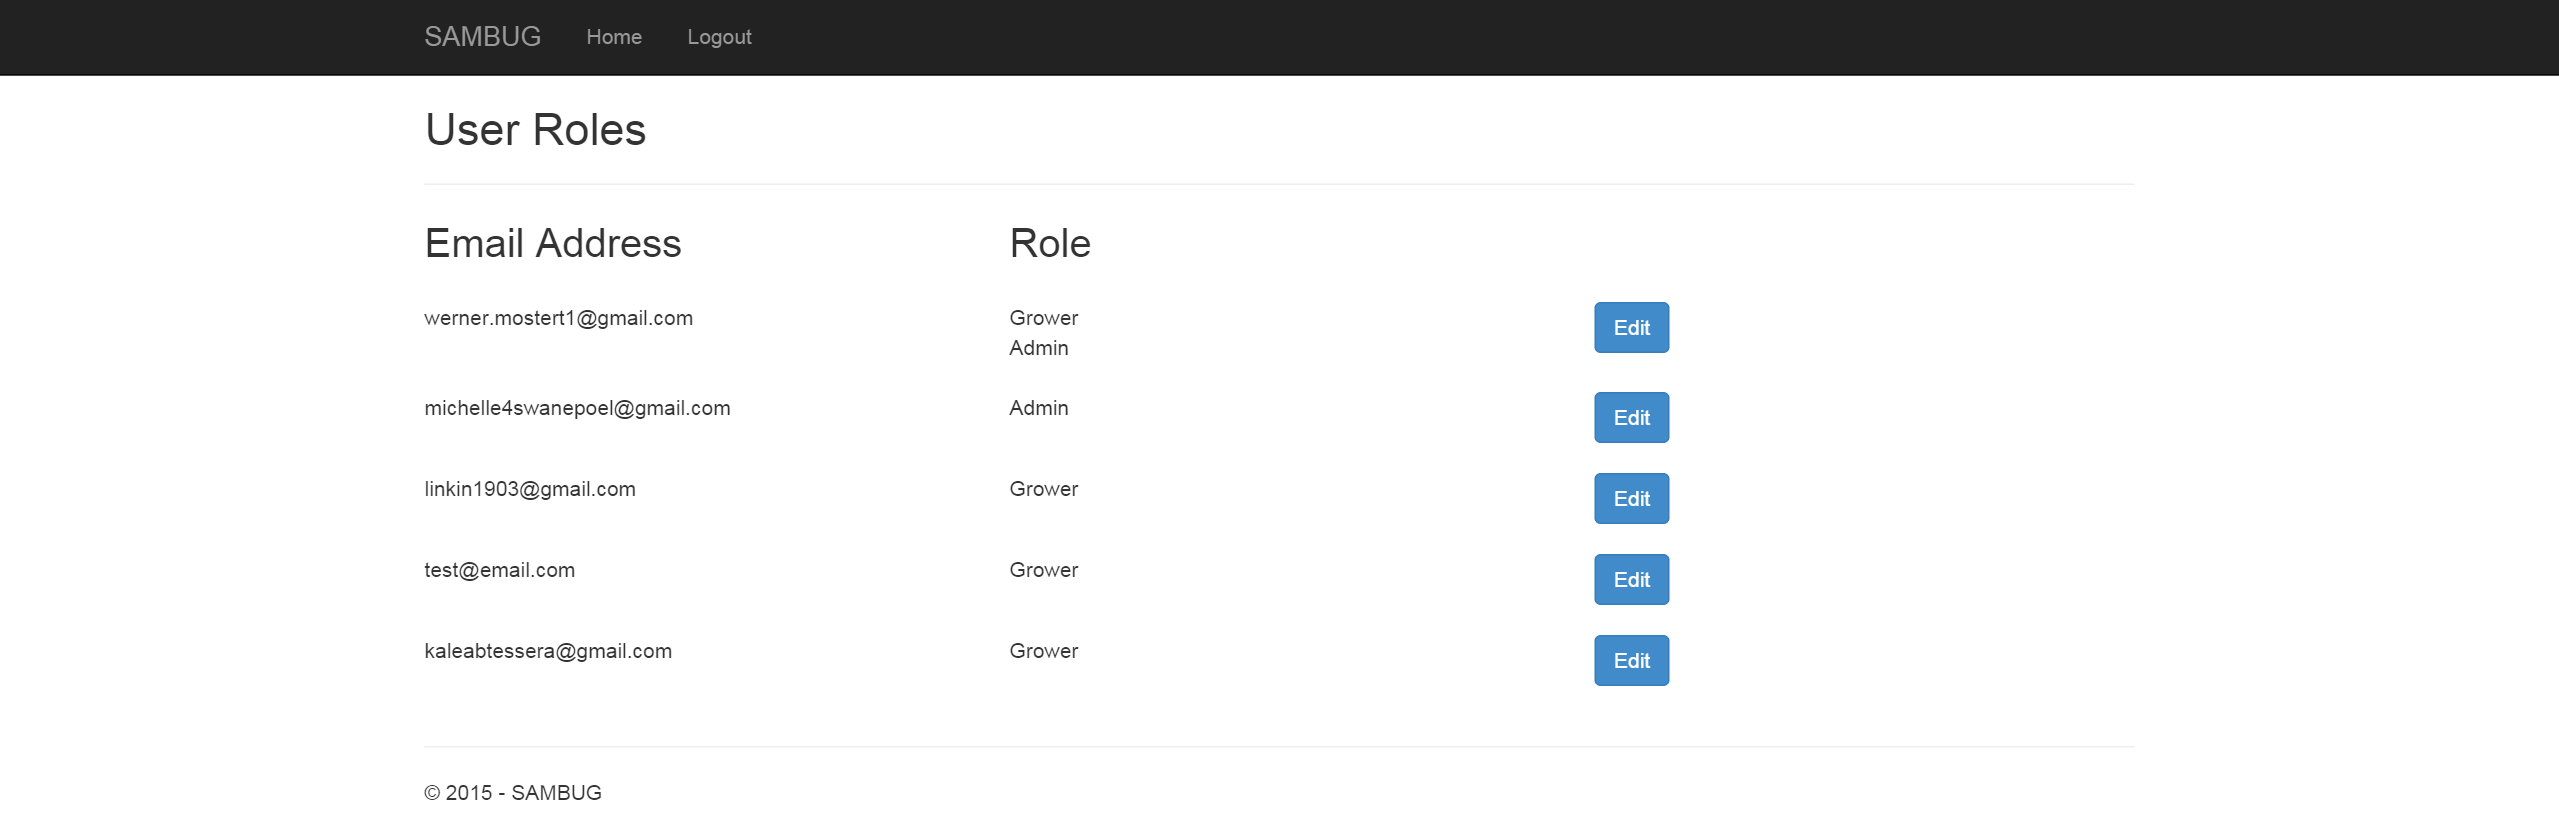
\includegraphics[width=\linewidth]{edituserroles.png}
	\end{center}
	On this page, a list of all users on the system will be shown with buttons to edit each user's roles. By clicking on the appropriate "Edit" button, the following modal dialog will appear in order for the selected user's roles to be changed:
		\begin{center}
			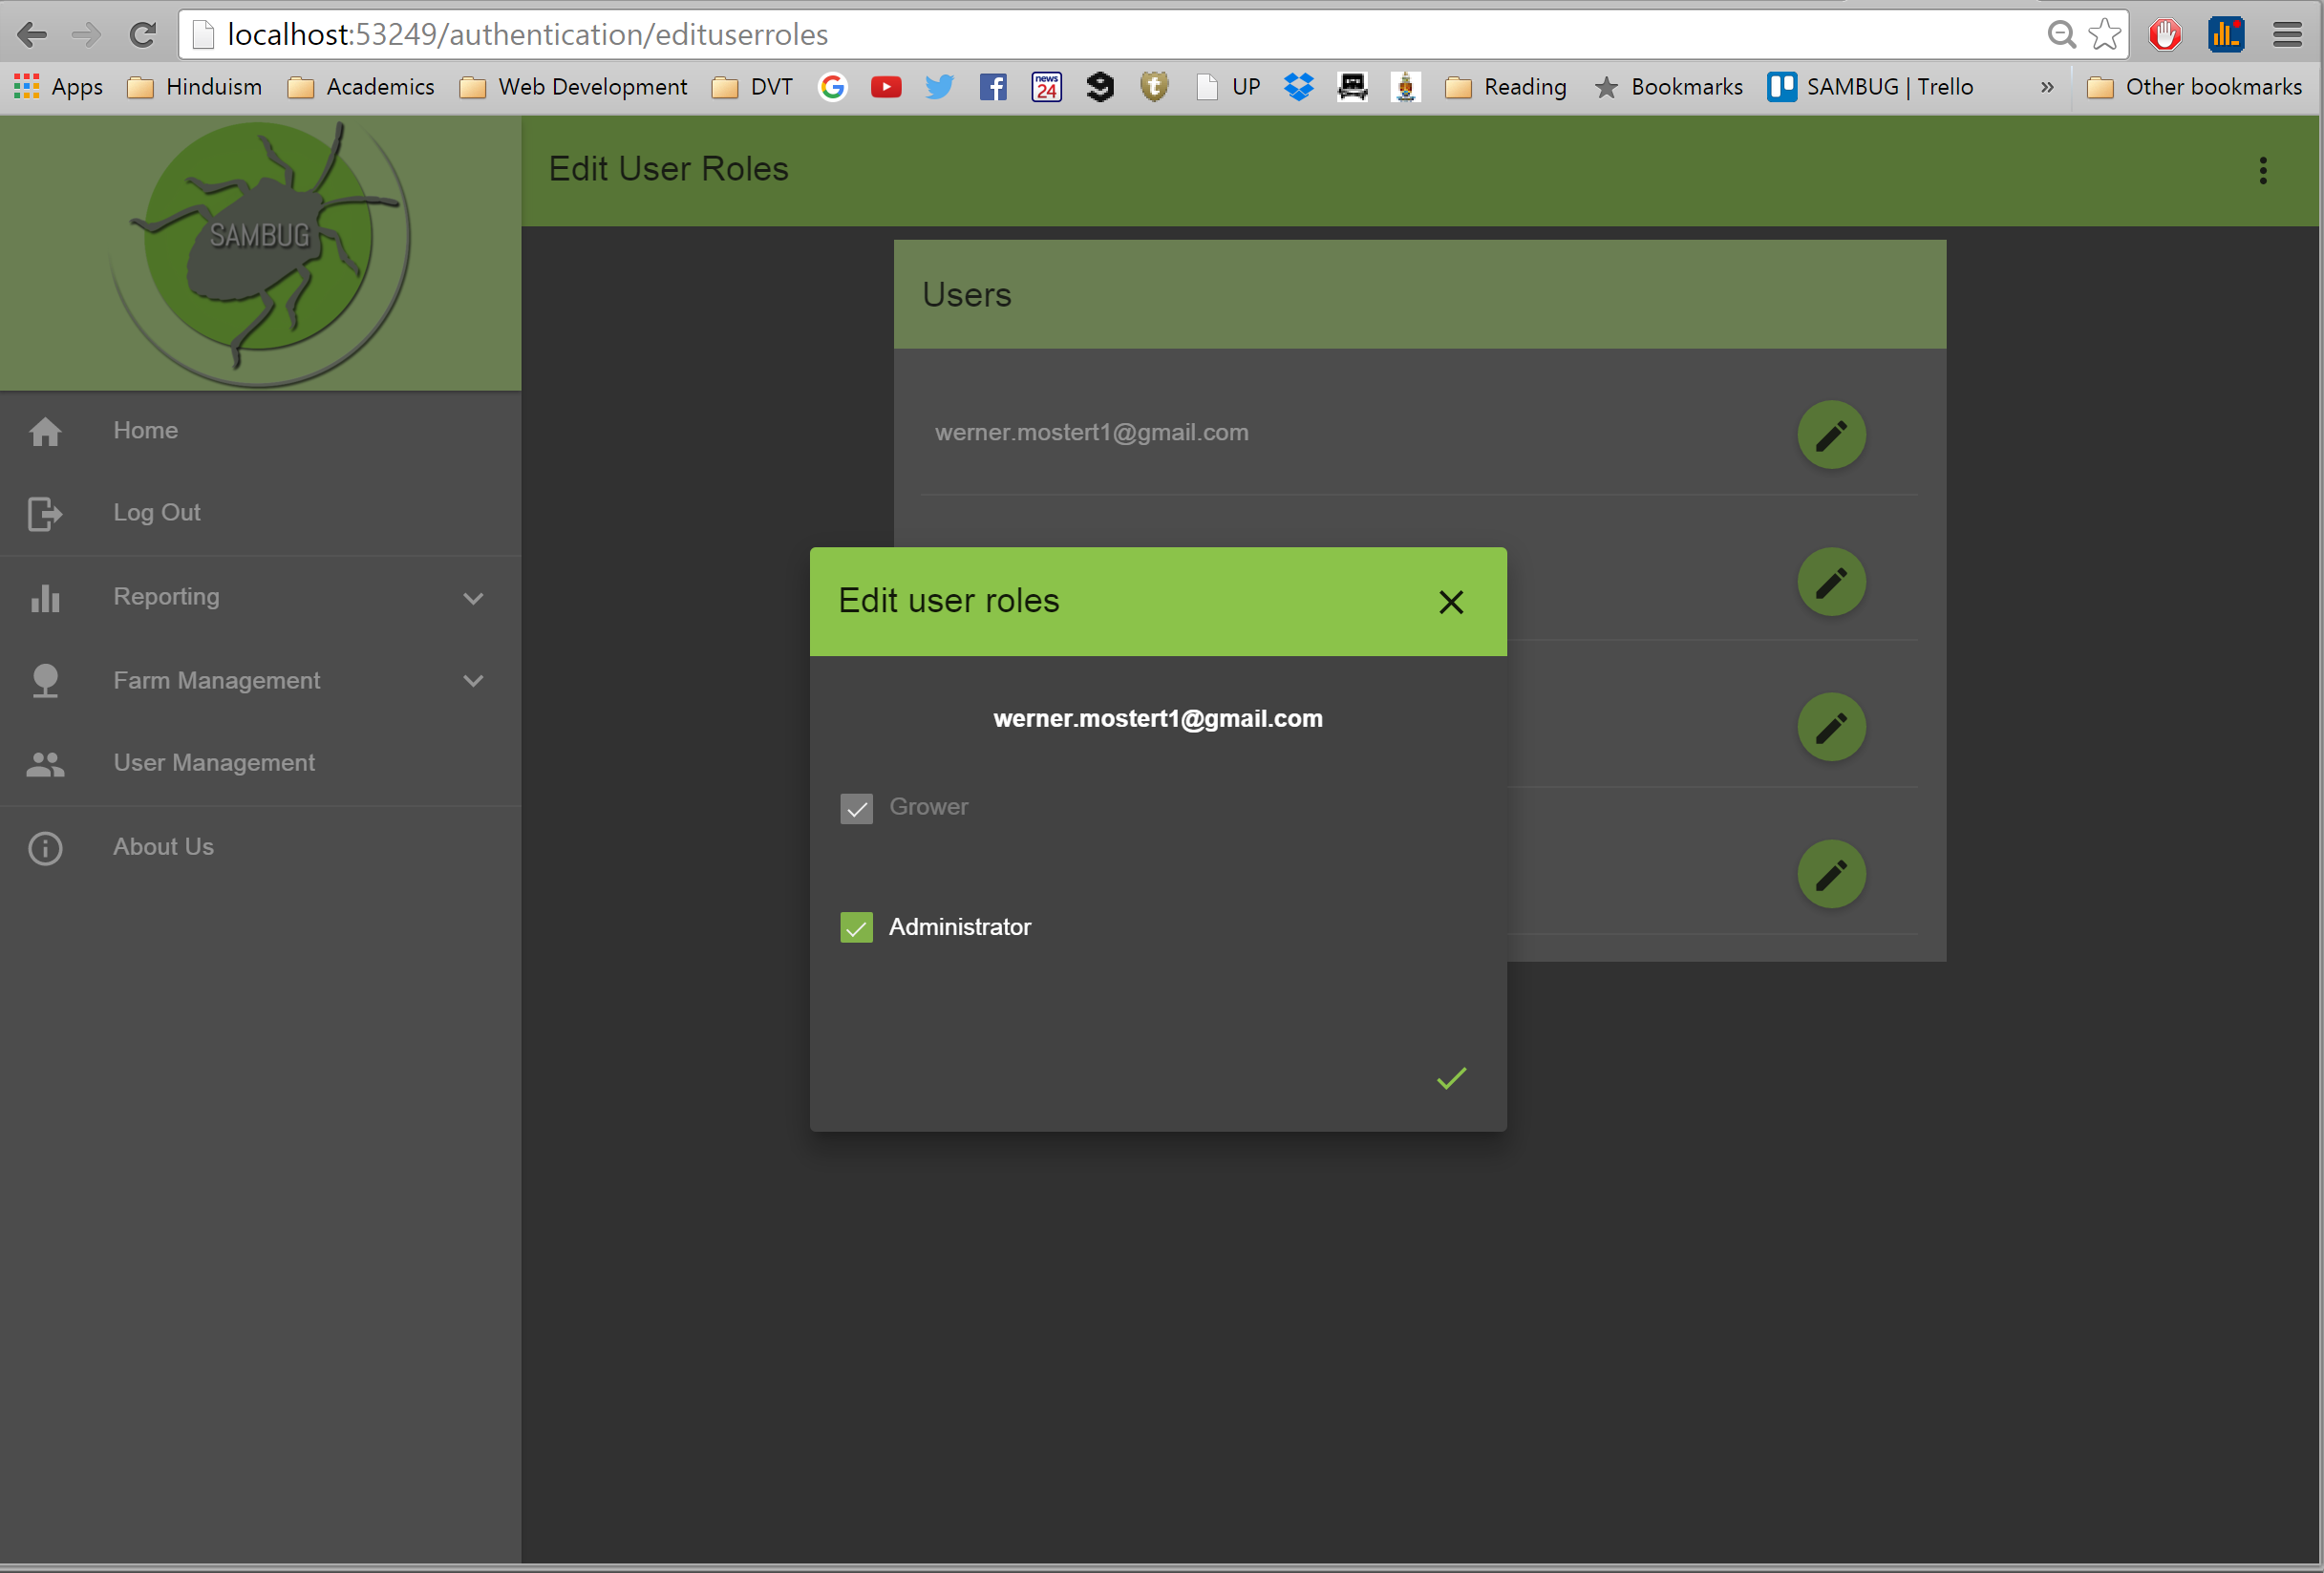
\includegraphics[width=\linewidth]{edituserrole.png} %TODO
		\end{center}
\item Finally, when the user is finished using the system, logout is completed by the simple task of clicking the "Logout" link found in the header bar of every page.
	\end{enumerate}
\subsection{Android Application}
	The application functions as a simple way for scouters to enter data. Follow these steps in order to use the application for scouting:
	\begin{enumerate}
		\item Open the application by clicking on the SAMBUGApp icon on your Android Device
		\item Once the Application has succesfully opened please login in with your registered username and password. If you have previously logged in, you will be automatically logged in in future. To log out, click on the logout button on the home screen. If you have not yet registered please go to the web page as described in the previous section in order to register. Click on Sign In to continue.
			\begin{center}
				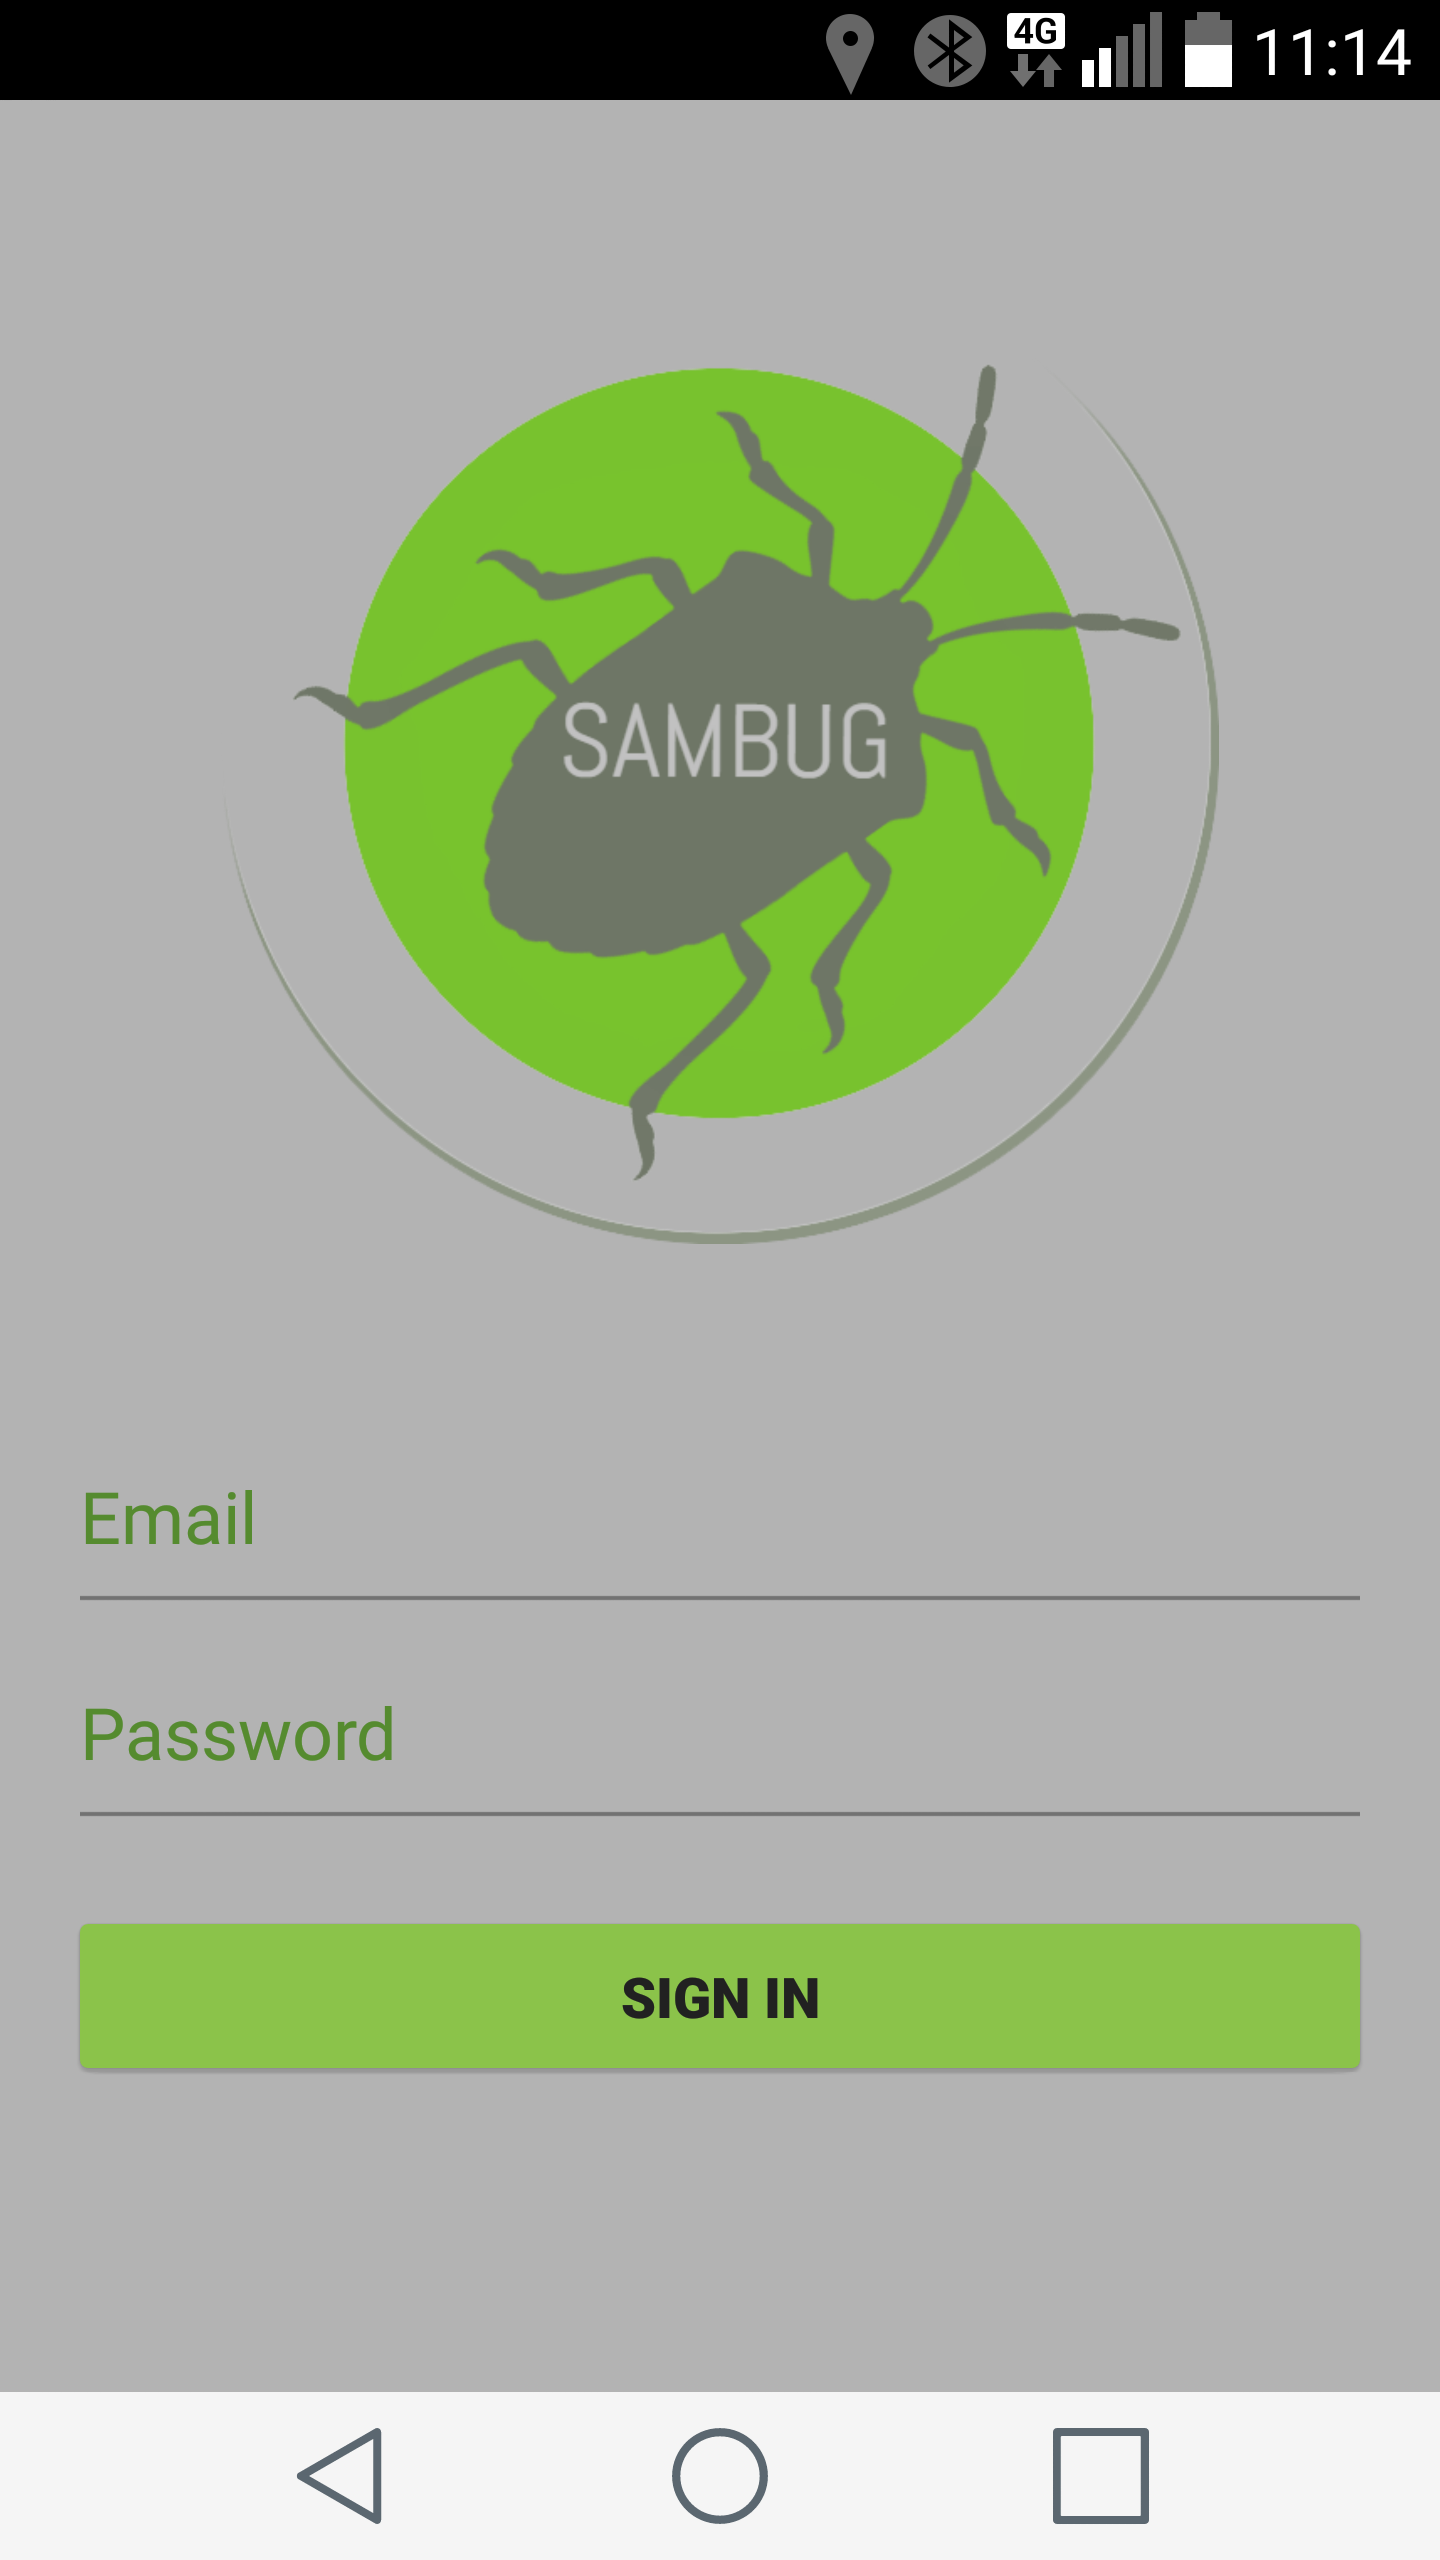
\includegraphics[scale=0.11]{login}
			\end{center}
		\item After successful login you will be presented with the following screen (The Home Screen):
			\begin{center}
				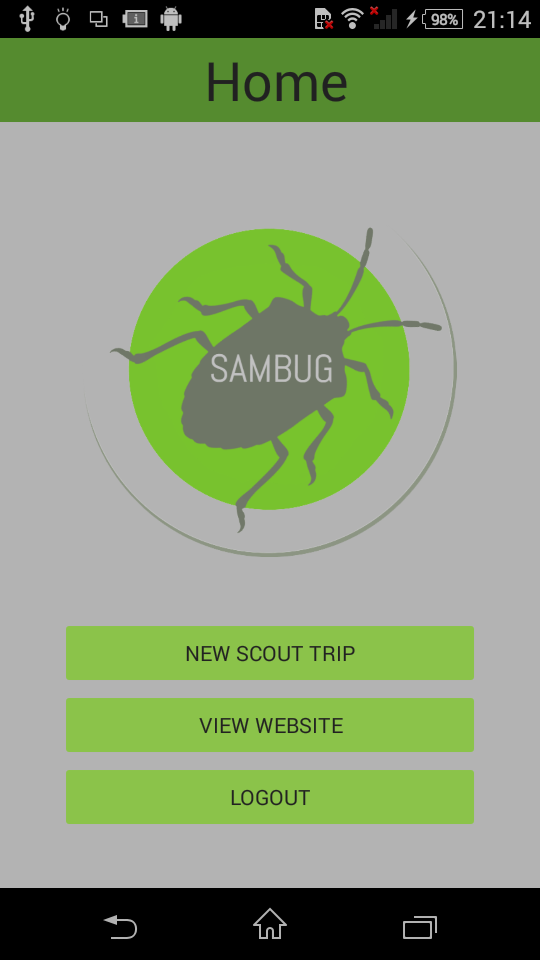
\includegraphics[scale=0.3]{home_nf}
			\end{center}
			Click on the [+] button on the top right hand corner of the screen in order to enter new scouting data.

	\item After being directed, select the block in which you are currently situated from the dropdown list at the top. After selecting the block, select the number of trees you have scouted in total. After entering the requested data, click on [ADD BUGS] to continue.
\begin{center}
				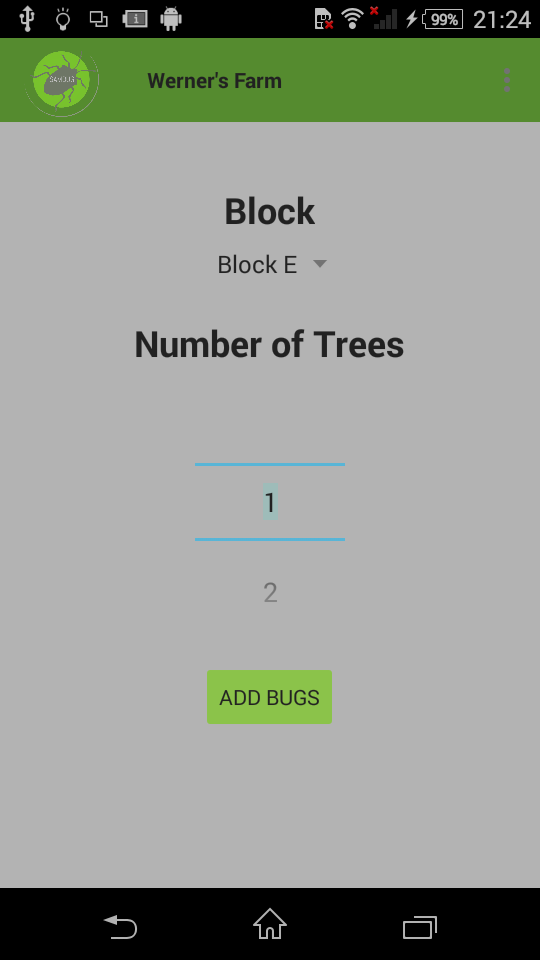
\includegraphics[scale=0.3]{enterdatainitial}
			\end{center}


 \item To start recording the different species of bugs that were found, click the [+] button in the middle lower area of the screen. In order to change the number of trees or block selection, click on the pencil button on the top right corner of the screen.
		\begin{center}
				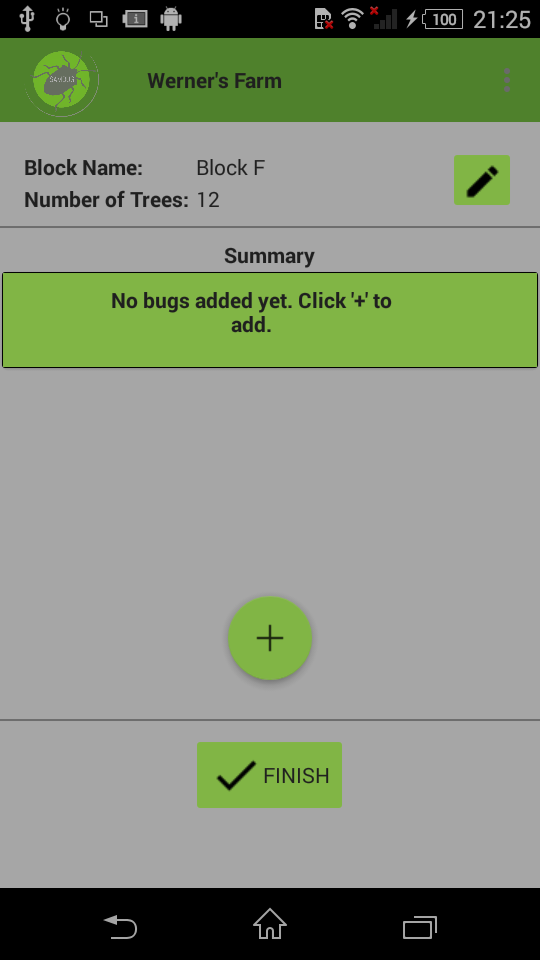
\includegraphics[scale=0.3]{enterdataempty}
			\end{center}

\item After click the [+], you will be requested to take a picture of a stinkbug. \textbf{\textit{For good results, place the stinkbug with it's back facing the camera on a white paper in natural light. Excessive shadows, blurred images and general bad image quality may affect automatic classification results. Please place the stinkbug in the center of the square drawn on-screen with the bug filling one to three quarters of the square.}}
	\begin{center}
				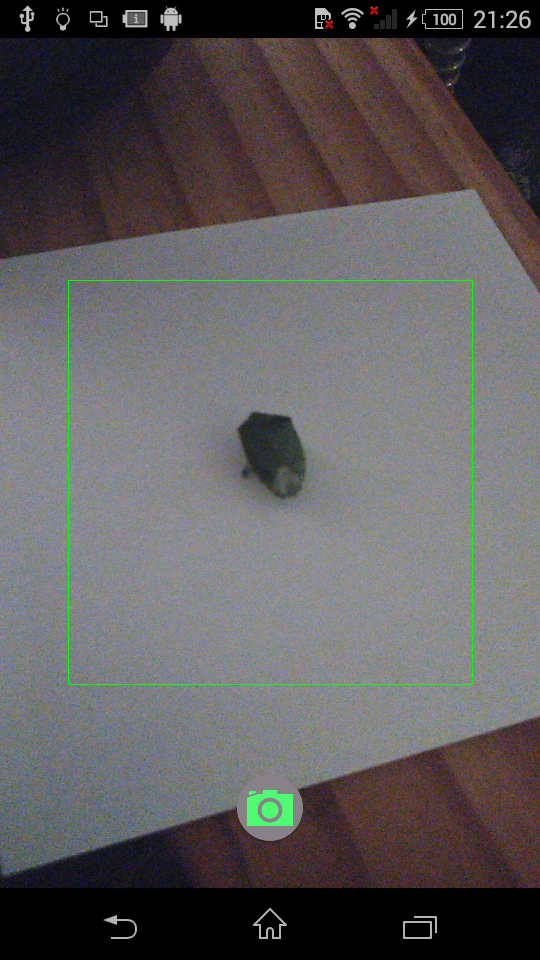
\includegraphics[scale=0.3]{captureimage}
	\end{center}


	\item Once a picture of the bug has been taken, your picture will appear on the left hand - top side of the screen. The application will immediatly attempt to determine the bug's species and lifestage. To have the application determine the species automatically again, click on the [CHOOSE AUTOMATICALLY] button at the top left corner. If you believe the choice was not accurate or if you prefer to choose the species yourself, select the specific bug type for the gallery from the bottom half of the screen. Once you are satisfied with your selection, click on [DONE].
	\begin{center}
				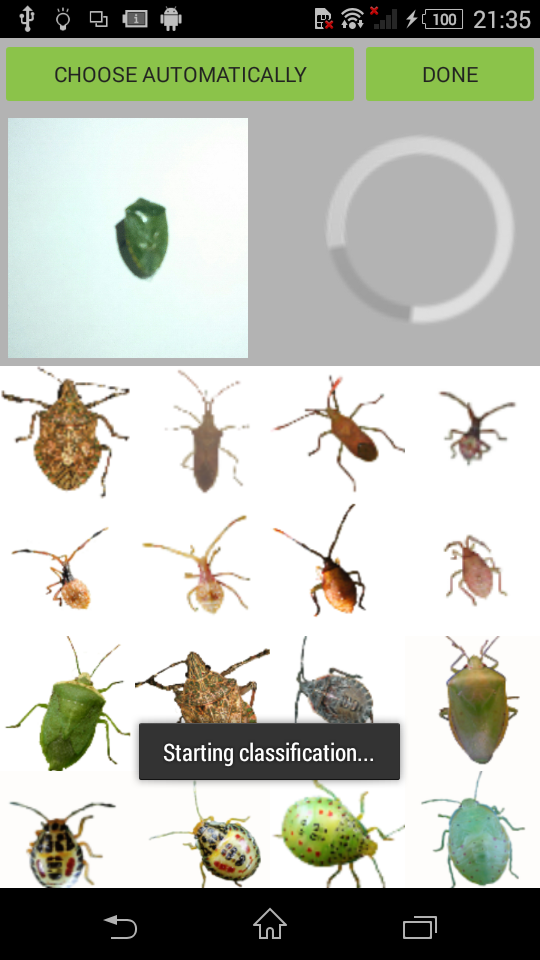
\includegraphics[scale=0.3]{identiftyclassifystart}
			\end{center}

\item Once [DONE] has been clicked a dialogue will require that the number of bugs are recorded. Please enter this amount and click [FINISH].
\begin{center}
				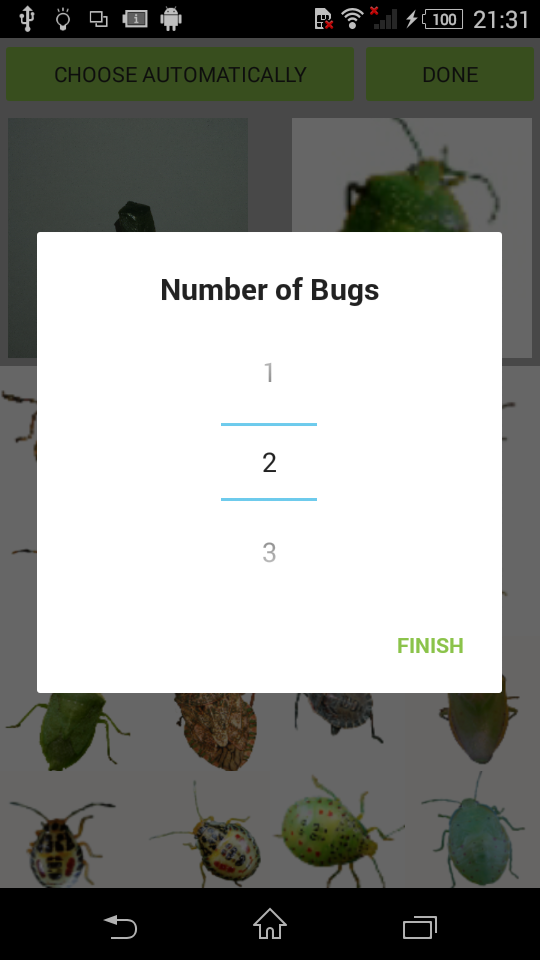
\includegraphics[scale=0.3]{identifychoosenumber}
			\end{center}

\item Once you are done with selecting the species, repeat until you have identified and counted all the bugs. Your results may look as below for a single entry:

\begin{center}
				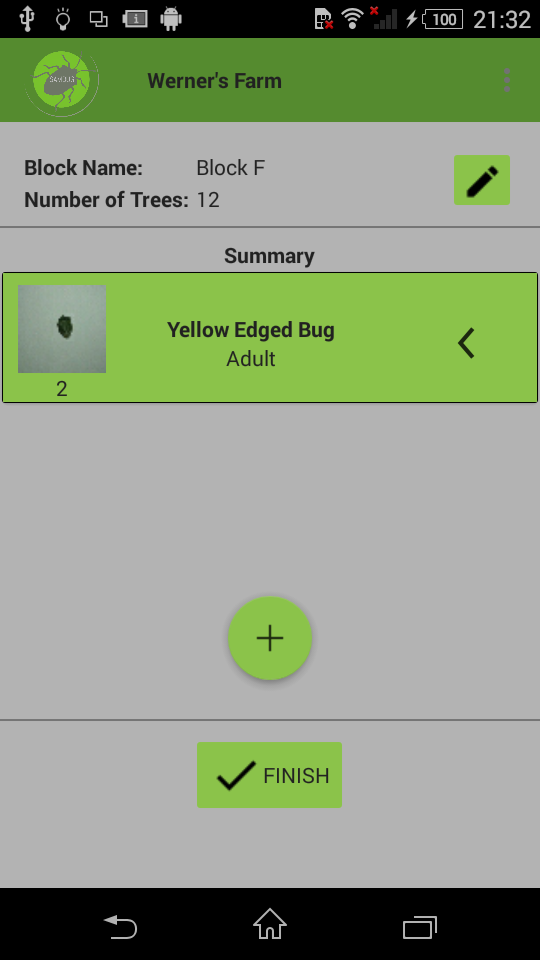
\includegraphics[scale=0.3]{enterdatafinal}
			\end{center}

\item When all the bugs have been identified and counted click on [DONE]. One is directed to a screen showing the collective scouting information as below:

\begin{center}
				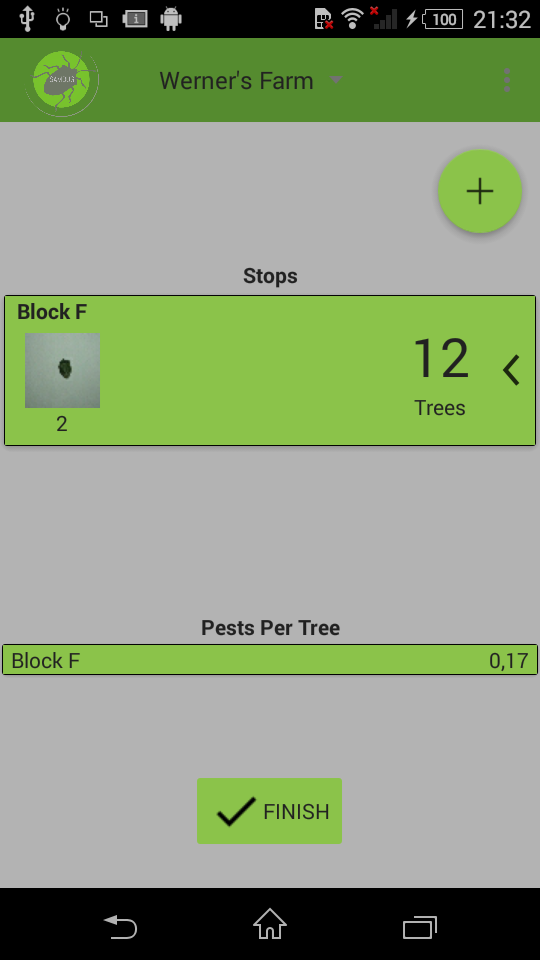
\includegraphics[scale=0.3]{scouttripfinal}
\end{center}

\item If you have moved to a different block and/or wish to continue scouting repeat the steps above. When you are done, click [FINISH] and your data will soon be available to the Farmer on the web page.
\begin{center}
				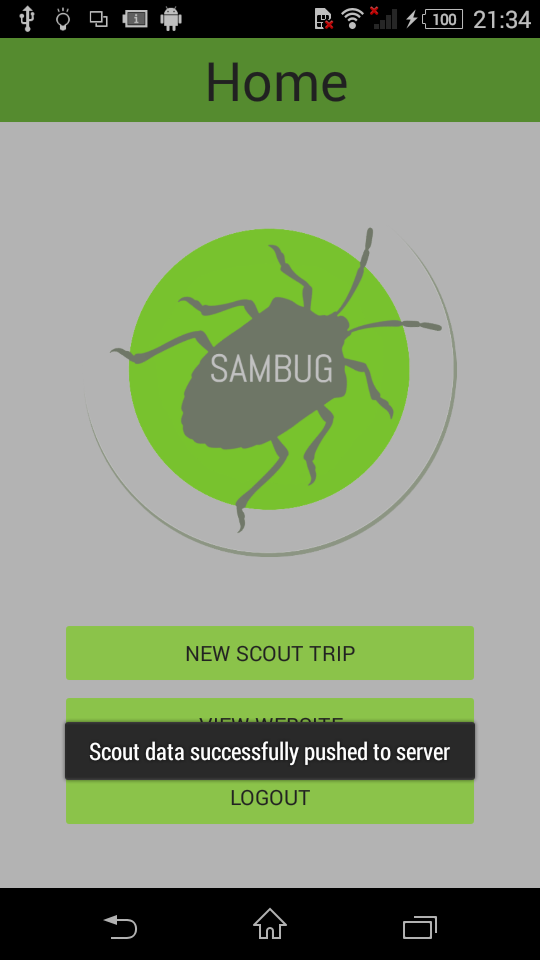
\includegraphics[scale=0.3]{homedatapushed}
\end{center}
\end{enumerate}


\section{Troubleshooting}
	\begin{itemize}
		\item Improve Location Accuracy - the User needs to switch on their gps to make use of the gps tracking and persist this to the db. If GPS is not on, this pop-up will appear prompting the user to switch their GPS on. \newline
		Suggested Action: Select the option to switch the GPS on. \newline
		
		\begin{center}
				\includegraphics[scale=0.3]{CAPTURE}
		\end{center}
		
		\item Unable to use flash. Battery too low. - the user needs to have enough battery to take a picture by making use of the camera api. \newline
		Suggested Action: Charge the phone and try again with more battery life. \newline
		
		\begin{center}
				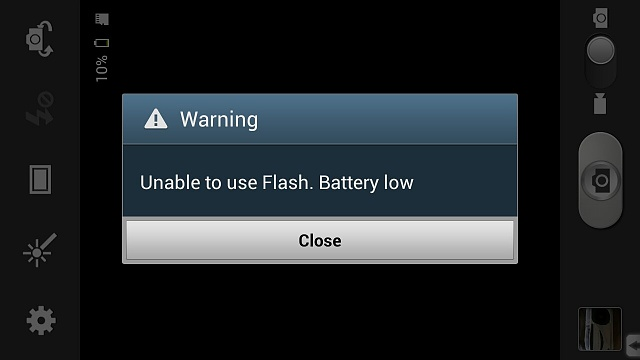
\includegraphics[scale=0.3]{Battery_Low}
		\end{center}
	\end{itemize}

\end{document}

%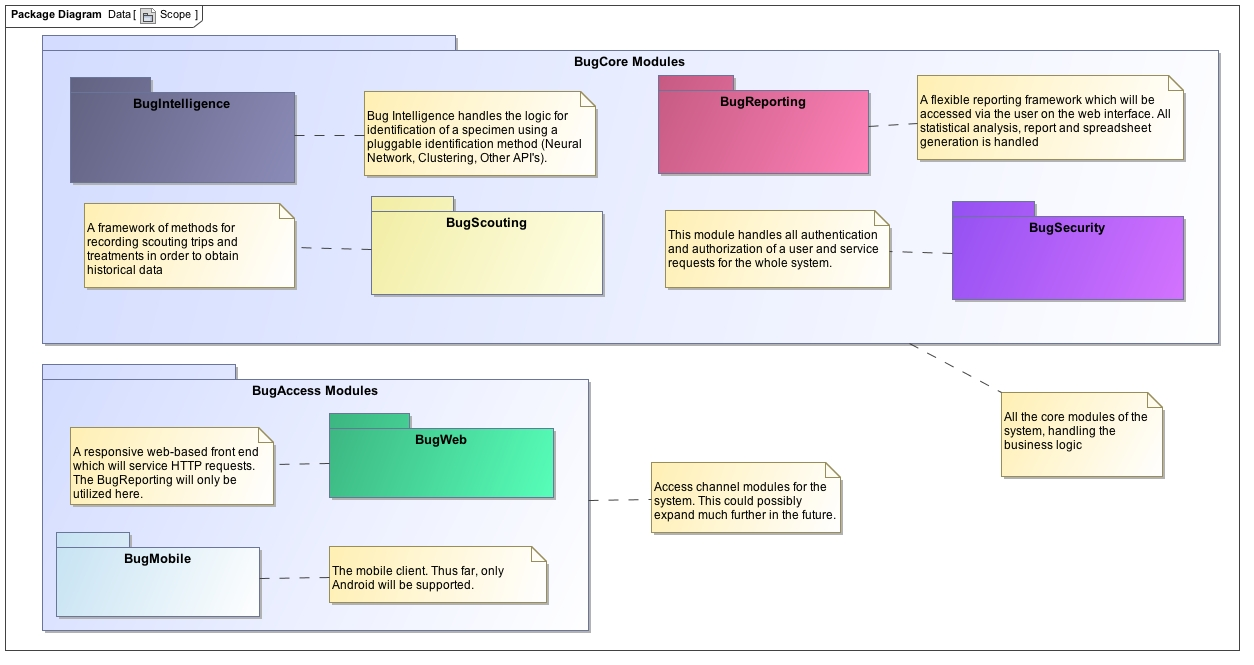
\includegraphics[width=\linewidth]{scope}